\documentclass{beamer}
\usepackage{listings}
\usepackage{graphicx}
\usepackage{bm}
\usepackage{amsmath,amssymb,xcolor,graphicx,url,natbib}
\usepackage{amsthm}
\usepackage{subfigure} % allow matrices of figures
\bibliographystyle{abbrv}
\usepackage{float}
\usepackage{animate}
\usepackage{pgffor}
\usepackage{hyperref}

\newcommand{\bd}{\begin{description}} 
\newcommand{\ed}{\end{description}} 
\newcommand{\bi}{\begin{itemize}} 
\newcommand{\ei}{\end{itemize}} 

%\logo{
\includegraphics[width=2cm]{plots/TAB_col_white_background.eps}}

\addtobeamertemplate{frametitle}{}{
	\vspace{-0.6cm}\hfill\raisebox{-0.65ex}{
\includegraphics[height=1cm]{plots/TAB_col_white_background.eps}}}

\setbeamertemplate{footline}{\scriptsize
	\hfill \insertframenumber
}


\title{\fontsize{14pt}{12pt}\selectfont Elastic fibres in shear flows can maintain steady orientations}
%\subtitle{}
\author{
	Hao Ye \\ \textit{Department of Mathematics} \\
	\vspace{0.5cm} 
	Supervisors: \\Matthias Heil, Draga Pihler-Puzović
}
%\date{\tiny Please update course code, project number, name and Student ID!}
\begin{document}

\begin{frame}[plain] 
	\maketitle 
	
	%\vfill 
	
	\begin{center}
		
\includegraphics[height=1.2cm]{plots/TAB_col_white_background.eps} 
	\end{center}
\end{frame}

%%%%%%%%%%%%%%%%%%%%%%%%%%%%%%%%%%%%%%%%%%%%%%%%%%%%%%%%%%%%%%%%%%%%%%

%\frame{\titlepage}

%%%%%%%%%%%%%%%%%%%%%%%%%%%%%%%%%%%%%%%%%%%%%%%%%%%%%%%%%%%%%%%%%%%%%%

\begin{frame}
	\frametitle{Motivation: particles in shear flow}
	\begin{overlayarea}{\textwidth}{\textheight}
		\vspace{-0.2cm}
    	\begin{figure}
			\begin{minipage}{0.4\linewidth}
				\centering
				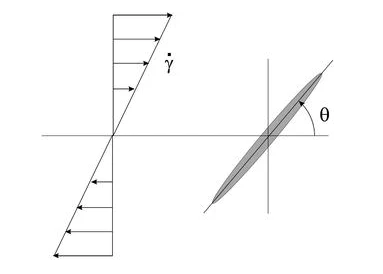
\includegraphics[width=\linewidth]{plots/application2.png} 
			 \centering \scriptsize A rigid ellipsoid \cite{yasuda2004experimental}.
			\end{minipage}
		\begin{minipage}{0.5\linewidth}
			\centering
			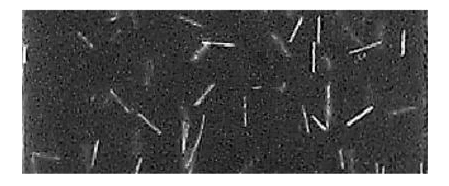
\includegraphics[width=\linewidth]{plots/application2_2.png} 
			\centering \scriptsize Vinylon fibers (paper industry) \cite{yasuda2004experimental}.
		\end{minipage}\vspace{0.5cm}
	\begin{minipage}{0.3\linewidth}
		\centering
		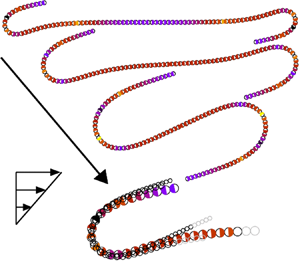
\includegraphics[width=\linewidth]{plots/application6.png} 
		\centering \scriptsize Elongated elastic fibres \cite{zuk2021universal}.
	\end{minipage}
		\begin{minipage}{0.32\linewidth}
		\centering
		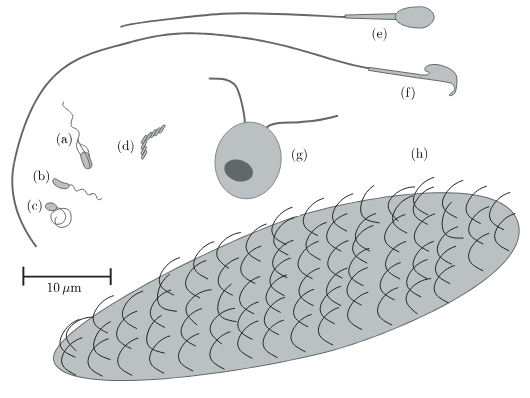
\includegraphics[width=\linewidth]{plots/application1.png} 
		\centering \scriptsize Sketches of microscopic swimmers, to scale \cite{lauga2009hydrodynamics}.
	\end{minipage}
		\begin{minipage}{0.35\linewidth}
	\centering
	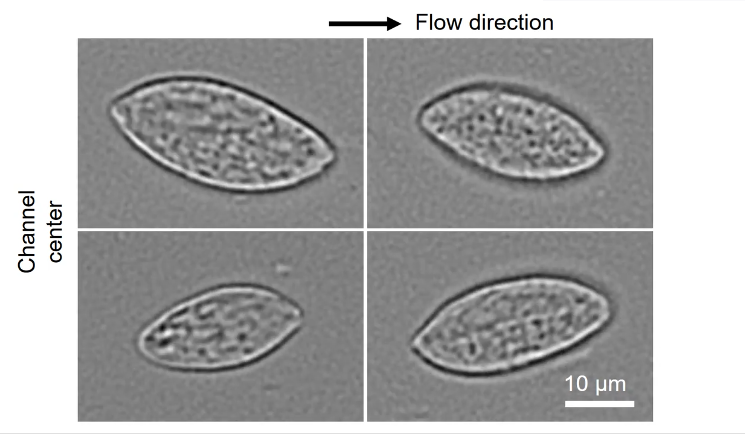
\includegraphics[width=\linewidth]{plots/application5.png}
	\centering \scriptsize Tank-treading motion of cells (video) \cite{gerum2022viscoelastic}.
\end{minipage}
		\end{figure}
	\end{overlayarea}
\end{frame}

%%%%%%%%%%%%%%%%%%%%%%%%%%%%%%%%%%%%%%%%%%%%%%%%%%%%%%%%%%%%%%%%%%%%%%

\begin{frame}
	\frametitle{Introduction: Jeffery orbits}
	\begin{overlayarea}{\textwidth}{\textheight}
		\vspace{-0.2cm}
	\begin{columns}
	\column{.6\textwidth}
	\begin{figure}[htb]
		\begin{center}
			% specify width as 80% of the width of the text on the page
			% we can also specify a width in centimetres, e.g. [width=8cm]
			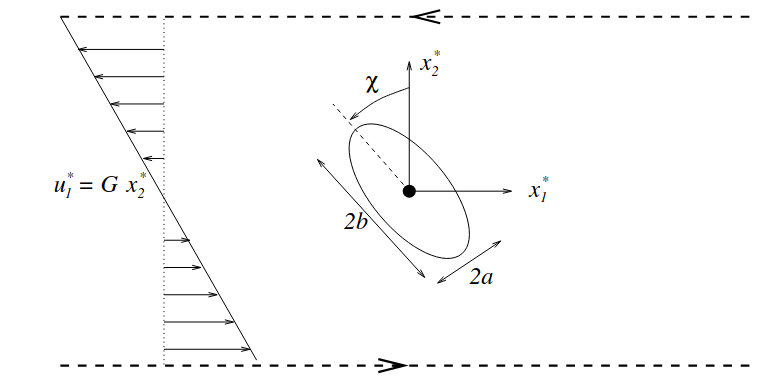
\includegraphics[width=1\textwidth]{plots/jeffery.png}
		\end{center}
		%	\setlength{\abovecaptionskip}{-0.5 cm}
	\end{figure}
	\column{.55\textwidth}
	\small
	\bi
	\item Jeffery (1922): periodic tumbling motion of rigid ellipsoidal particles in shear flow.
	\ei 
\end{columns}
\vspace{0.5cm}
\bi 
\item If vorticity $\omega\neq 0$, typically particles will undergo a periodic rotation (Jeffery orbits).
	\item The periodic motion depends on the particle shapes ($\&$ initial conditions).
\ei
		%\vspace{0.1cm}
	\end{overlayarea}
\end{frame}

%%%%%%%%%%%%%%%%%%%%%%%%%%%%%%%%%%%%%%%%%%%%%%%%%%%%%%%%%%%%%%%%%%%%%%

\begin{frame}
	\frametitle{Introduction: Jeffery orbits}
	\begin{overlayarea}{\textwidth}{\textheight}
		\vspace{-0.2cm}
		\begin{columns}
			\column{.6\textwidth}
			\begin{figure}[htb]
				\begin{center}
					% specify width as 80% of the width of the text on the page
					% we can also specify a width in centimetres, e.g. [width=8cm]
					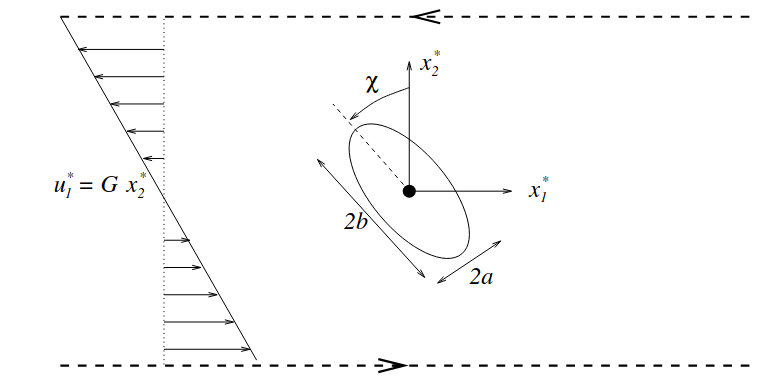
\includegraphics[width=1\textwidth]{plots/jeffery.png}
				\end{center}
				%	\setlength{\abovecaptionskip}{-0.5 cm}
			\end{figure}
			\column{.55\textwidth}
			\small
			\bi
			\item Jeffery (1922): periodic tumbling motion of rigid ellipsoidal particles in shear flow.
			\ei 
		\end{columns}
		\vspace{0.5cm}
		\bi 
		\item If \alert{vorticity $\omega\neq 0$}, typically particles will undergo a periodic \alert{rotation} (Jeffery orbits).
		\item The periodic motion depends on the particle shapes ($\&$ initial conditions).
		\ei
		%\vspace{0.1cm}
	\end{overlayarea}
\end{frame}

%%%%%%%%%%%%%%%%%%%%%%%%%%%%%%%%%%%%%%%%%%%%%%%%%%%%%%%%%%%%%%%%%%%%%%

%%%%%%%%%%%%%%%%%%%%%%%%%%%%%%%%%%%%%%%%%%%%%%%%%%%%%%%%%%%%%%%%%%%%%%

\begin{frame}
	\frametitle{Introduction: Jeffery orbits}
	\begin{overlayarea}{\textwidth}{\textheight}
		\vspace{-0.2cm}
		\begin{columns}
			\column{.6\textwidth}
			\begin{figure}[htb]
				\begin{center}
					% specify width as 80% of the width of the text on the page
					% we can also specify a width in centimetres, e.g. [width=8cm]
					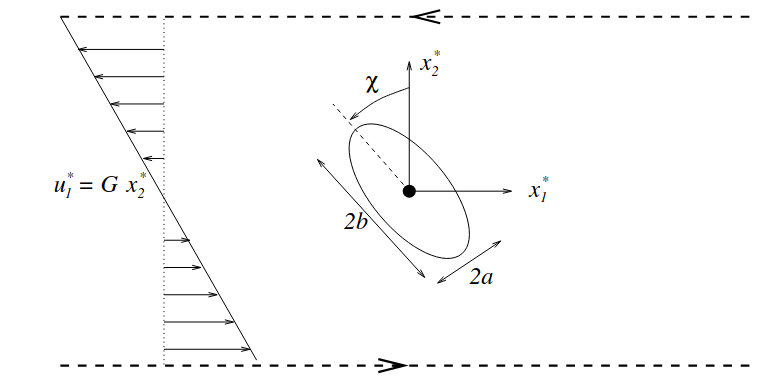
\includegraphics[width=1\textwidth]{plots/jeffery.png}
				\end{center}
				%	\setlength{\abovecaptionskip}{-0.5 cm}
			\end{figure}
			\column{.55\textwidth}
			\small
			\bi
			\item Jeffery (1922): periodic tumbling motion of rigid ellipsoidal particles in shear flow.
			\ei 
		\end{columns}
		\vspace{0.5cm}
		\bi 
		\item If \alert{vorticity $\omega\neq 0$}, typically particles will undergo a periodic \alert{rotation} (Jeffery orbits).
		\item The periodic motion depends on the particle shapes ($\&$ initial conditions).
		\ei
		\centering \LARGE \colorbox{yellow}{Is it true for all particles?}
		%\vspace{0.1cm}
	\end{overlayarea}
\end{frame}

%%%%%%%%%%%%%%%%%%%%%%%%%%%%%%%%%%%%%%%%%%%%%%%%%%%%%%%%%%%%%%%%%%%%%%


\begin{frame}
	\frametitle{No,it isn't; boomerang-shaped particles}
	\begin{overlayarea}{\textwidth}{\textheight}
		\vspace{-0.5cm}
		\footnotesize Roggeveen J V, Stone H A. JFM (2022), 939: A23.\vspace{-0.2cm}
		\begin{columns}
		\column{.55\textwidth}\vspace{0.5cm}
		\begin{figure}[htb]
			\begin{center}
				% specify width as 80% of the width of the text on the page
				% we can also specify a width in centimetres, e.g. [width=8cm]
				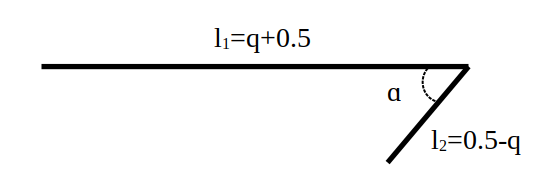
\includegraphics[width=1\textwidth]{plots/geometry2.png}
			\end{center}
			%	\setlength{\abovecaptionskip}{-0.5 cm}
		\end{figure}
		\column{.6\textwidth}\vspace{-1.7cm}
		\small
		\bi
		\item $q \in [0,0.5), \alpha \in (0,2\pi)$.
		\ei
		\end{columns}
	\end{overlayarea}
\end{frame}

%%%%%%%%%%%%%%%%%%%%%%%%%%%%%%%%%%%%%%%%%%%%%%%%%%%%%%%%%%%%%%%%%%%%%%


\begin{frame}
	\frametitle{No,it isn't; boomerang-shaped particles}
	\begin{overlayarea}{\textwidth}{\textheight}
		\vspace{-0.5cm}
		\footnotesize Roggeveen J V, Stone H A. JFM (2022), 939: A23.\vspace{-0.2cm}
		\begin{columns}
			\column{.55\textwidth}
			\begin{figure}[htb]
				\begin{center}
					% specify width as 80% of the width of the text on the page
					% we can also specify a width in centimetres, e.g. [width=8cm]
					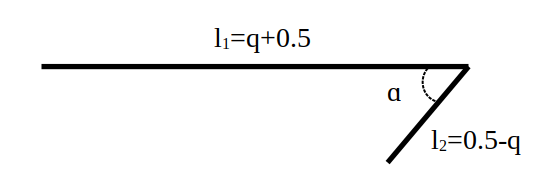
\includegraphics[width=1\textwidth]{plots/geometry2.png}
				\end{center}
				%	\setlength{\abovecaptionskip}{-0.5 cm}
			\end{figure}
			\column{.6\textwidth}
			\small
			\bi
			\item $q \in [0,0.5), \alpha \in (0,2\pi)$.
			\item Extreme cases:
			$
			\label{eqn:1}
			\left.
			\begin{aligned}
				&\alpha=0,\pi \\
				&	q=0.5
			\end{aligned}
			\right\}\Longrightarrow \text{straight rod},$ 
			
			$q=0, \alpha \neq 0, \pi \Longrightarrow \text{same arm length}.
			$
			\ei 
		\end{columns}
		\vspace{0.1cm} \small
		\bi
		\item As $q$ increases, the short arm shortens while the long arm lengthens.
		\ei 
	\end{overlayarea}
\end{frame}

%%%%%%%%%%%%%%%%%%%%%%%%%%%%%%%%%%%%%%%%%%%%%%%%%%%%%%%%%%%%%%%%%%%%%%

\begin{frame}
	\frametitle{No,it isn't; boomerang-shaped particles}
	\begin{overlayarea}{\textwidth}{\textheight}
		\vspace{-0.5cm}
		\footnotesize Roggeveen J V, Stone H A. JFM (2022), 939: A23.\vspace{-0.2cm}
		\begin{columns}
			\column{.55\textwidth}
			\begin{figure}[htb]
				\begin{center}
					% specify width as 80% of the width of the text on the page
					% we can also specify a width in centimetres, e.g. [width=8cm]
					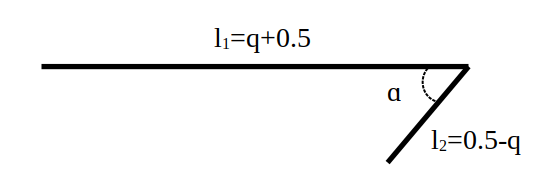
\includegraphics[width=1\textwidth]{plots/geometry2.png}
				\end{center}
				%	\setlength{\abovecaptionskip}{-0.5 cm}
			\end{figure}
			\column{.6\textwidth}
			\small
			\bi
			\item $q \in [0,0.5), \alpha \in (0,2\pi)$.
			\item Extreme cases:
			$
			\label{eqn:1}
			\left.
			\begin{aligned}
				&\alpha=0,\pi \\
				&	q=0.5
			\end{aligned}
			\right\}\Longrightarrow \text{straight rod},$ 
			
			$q=0, \alpha \neq 0, \pi \Longrightarrow \text{same arm length}.
			$
			\ei 
		\end{columns}
		\vspace{0.1cm} \small
		\bi
		\item As $q$ increases, the short arm shortens while the long arm lengthens.
		\ei  \vspace{-0.15cm}
		\begin{columns}
			\column{.55\textwidth}
			Results:
			\bi
			\item White: tumbling.
			\ei 
			\column{.5\textwidth}
			\begin{figure}[htb]
				\begin{center}
					% specify width as 80% of the width of the text on the page
					% we can also specify a width in centimetres, e.g. [width=8cm]
					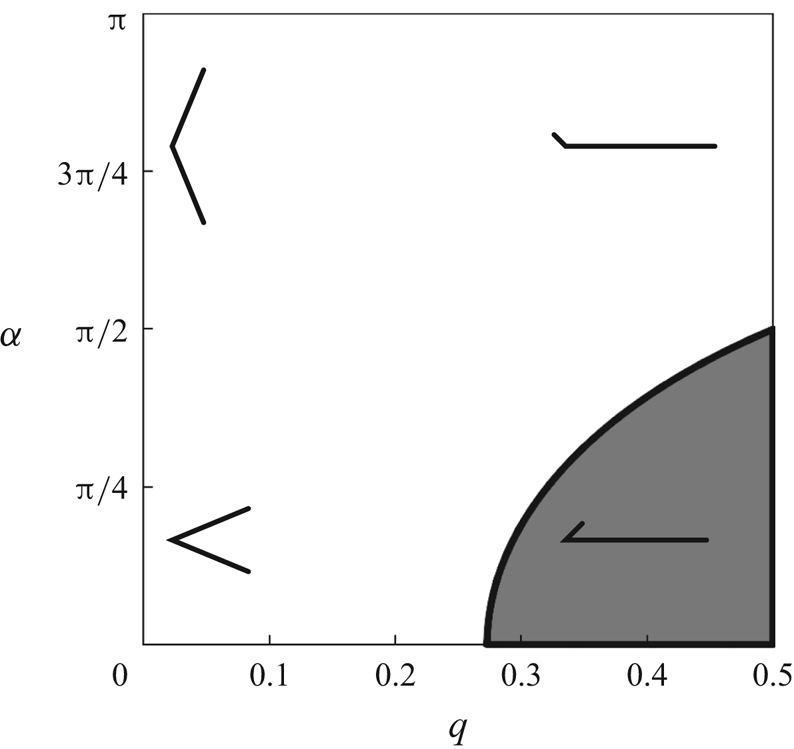
\includegraphics[width=0.85\textwidth]{plots/stone.png}
				\end{center}
				%	\setlength{\abovecaptionskip}{-0.5 cm}
			\end{figure}
		\end{columns}
	\end{overlayarea}
\end{frame}

%%%%%%%%%%%%%%%%%%%%%%%%%%%%%%%%%%%%%%%%%%%%%%%%%%%%%%%%%%%%%%%%%%%%%%




\begin{frame}
	\frametitle{No,it isn't; boomerang-shaped particles}
	\begin{overlayarea}{\textwidth}{\textheight}
\vspace{-0.5cm}
\footnotesize Roggeveen J V, Stone H A. JFM (2022), 939: A23.\vspace{-0.2cm}
\begin{columns}
	\column{.55\textwidth}
	\begin{figure}[htb]
		\begin{center}
			% specify width as 80% of the width of the text on the page
			% we can also specify a width in centimetres, e.g. [width=8cm]
			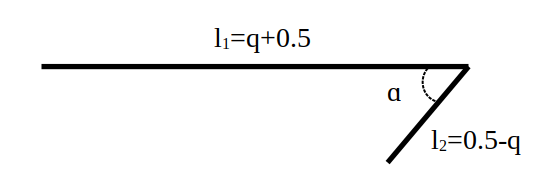
\includegraphics[width=1\textwidth]{plots/geometry2.png}
		\end{center}
		%	\setlength{\abovecaptionskip}{-0.5 cm}
	\end{figure}
	\column{.6\textwidth}
	\small
	\bi
	\item $q \in [0,0.5), \alpha \in (0,2\pi)$.
	\item Extreme cases:
	$
	\label{eqn:1}
	\left.
	\begin{aligned}
		&\alpha=0,\pi \\
		&	q=0.5
	\end{aligned}
	\right\}\Longrightarrow \text{straight rod},$ 
	
	$q=0, \alpha \neq 0, \pi \Longrightarrow \text{same arm length}.
	$
	\ei 
\end{columns}
\vspace{0.1cm} \small
\bi
\item As $q$ increases, the short arm shortens while the long arm lengthens.
\ei  \vspace{-0.15cm}
		\begin{columns}
			\column{.55\textwidth}
			Results:
			\bi
			\item White: tumbling. \item Grey: \colorbox{yellow}{\textbf{no rotation!}} 
			 (asymmetric, small $\alpha$). 
			\ei 
			\column{.5\textwidth}
			\begin{figure}[htb]
				\begin{center}
					% specify width as 80% of the width of the text on the page
					% we can also specify a width in centimetres, e.g. [width=8cm]
					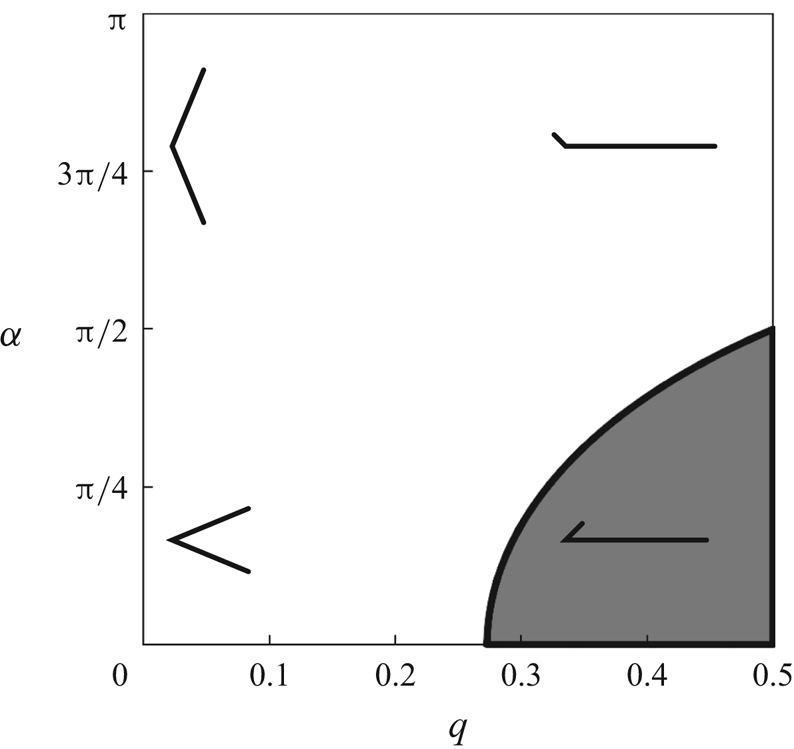
\includegraphics[width=0.85\textwidth]{plots/stone.png}
				\end{center}
				%	\setlength{\abovecaptionskip}{-0.5 cm}
			\end{figure}
		\end{columns}
	\end{overlayarea}
\end{frame}

%%%%%%%%%%%%%%%%%%%%%%%%%%%%%%%%%%%%%%%%%%%%%%%%%%%%%%%%%%%%%%%%%%%%%%


\begin{frame}
	\frametitle{No,it isn't; boomerang-shaped particles}
	\begin{overlayarea}{\textwidth}{\textheight}
		\vspace{-0.5cm}
		\footnotesize Roggeveen J V, Stone H A. JFM (2022), 939: A23.\vspace{-0.2cm}
		\begin{columns}
			\column{.6\textwidth}\vspace{-0.5cm}
			\begin{figure}[htb]
				\begin{center}
					% specify width as 80% of the width of the text on the page
					% we can also specify a width in centimetres, e.g. [width=8cm]
					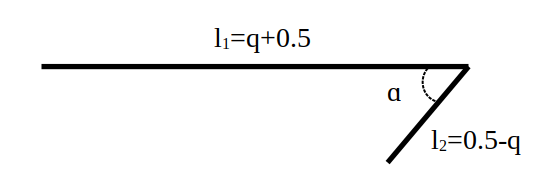
\includegraphics[width=0.85\textwidth]{plots/geometry2.png}
				\end{center}
				%	\setlength{\abovecaptionskip}{-0.5 cm}
			\end{figure}
			\column{.5\textwidth}
			\begin{figure}[htb]
			\begin{center}
				% specify width as 80% of the width of the text on the page
				% we can also specify a width in centimetres, e.g. [width=8cm]
				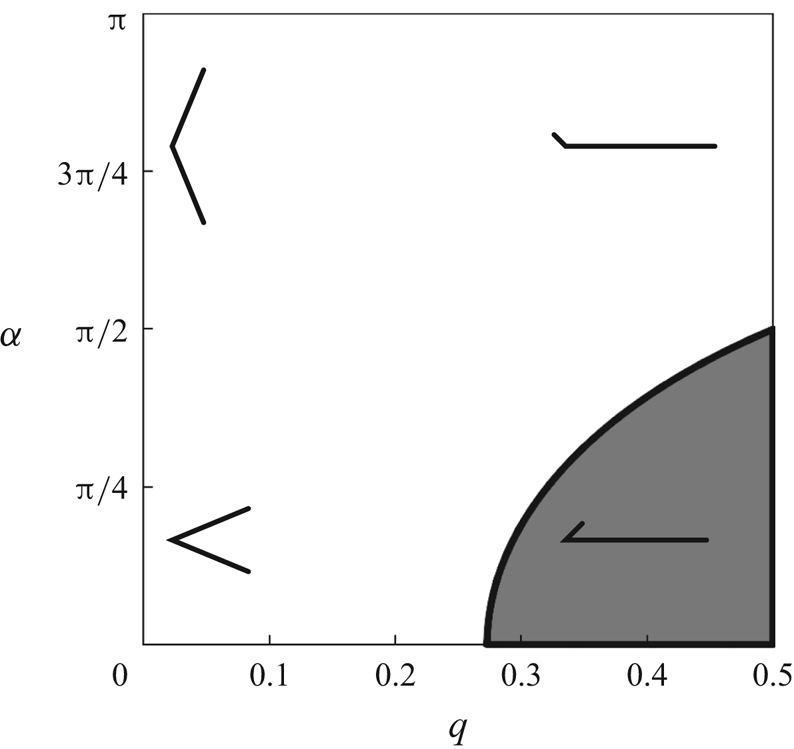
\includegraphics[width=0.85\textwidth]{plots/stone.png}
			\end{center}
			%	\setlength{\abovecaptionskip}{-0.5 cm}
		\end{figure}
		\end{columns}
	 \vspace{0.5cm}
		\begin{columns}
			\column{.55\textwidth}\small
			Results:
			\bi
			\item Four equilibria.
			\item Two stable, two unstable. 
			\item Persistent cross-streamline drift.
			\ei \vspace{0.5cm}
			\column{.6\textwidth}
			\vspace{-1cm}
			\begin{figure}[htb]
				\begin{center}
					% specify width as 80% of the width of the text on the page
					% we can also specify a width in centimetres, e.g. [width=8cm]
					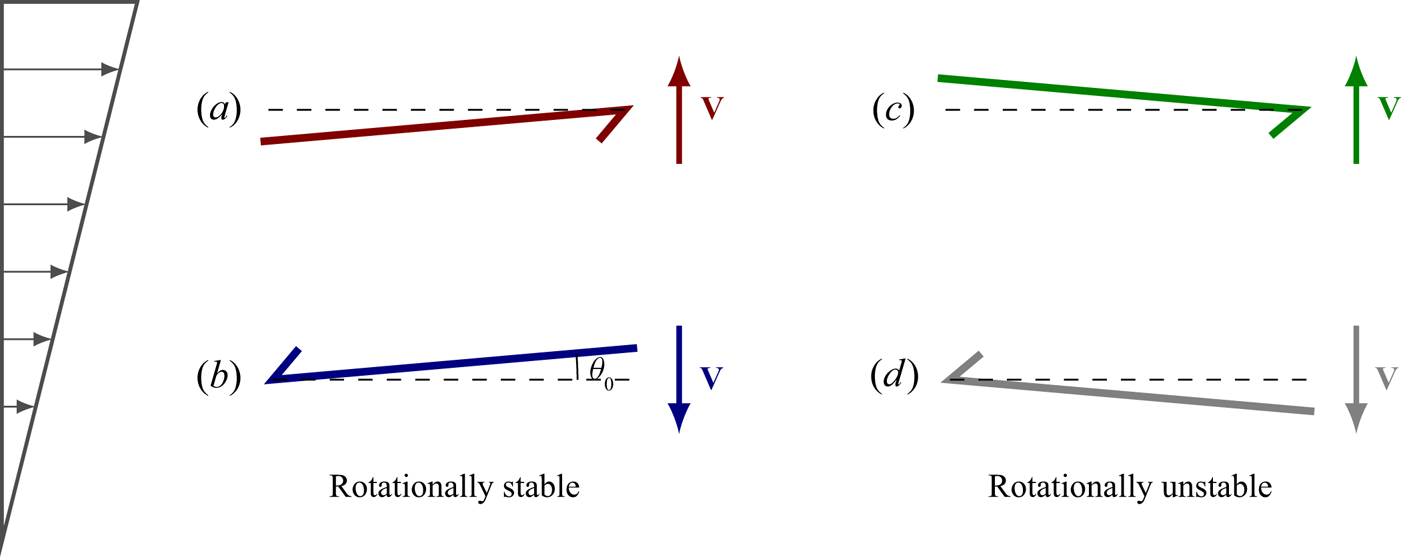
\includegraphics[width=1\textwidth]{plots/stone3.png}
				\end{center}
				%	\setlength{\abovecaptionskip}{-0.5 cm}
			\end{figure}
		\end{columns}
	\end{overlayarea}
\end{frame}

%%%%%%%%%%%%%%%%%%%%%%%%%%%%%%%%%%%%%%%%%%%%%%%%%%%%%%%%%%%%%%%%%%%%%%


\begin{frame}
	\frametitle{Theory: slender body theory}
	\begin{overlayarea}{\textwidth}{\textheight}
		\vspace{-0.8cm}
		\begin{columns}
			\column{.6\textwidth}	
			\begin{figure}[htb]
				\begin{center}
					% specify width as 80% of the width of the text on the page
					% we can also specify a width in centimetres, e.g. [width=8cm]
					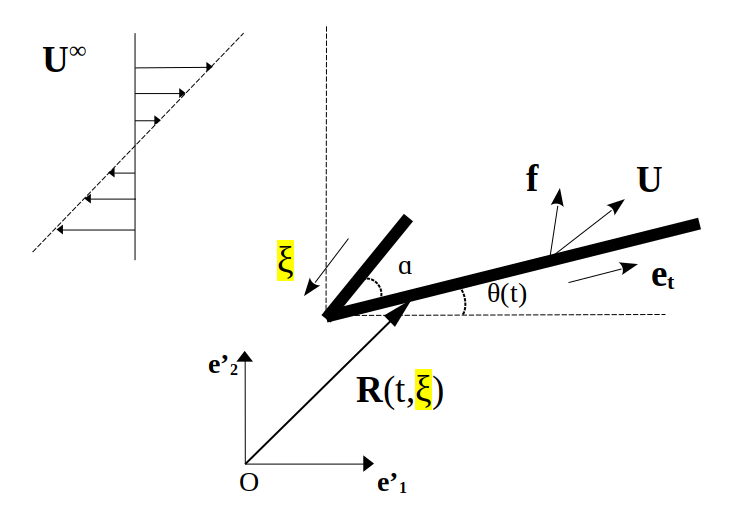
\includegraphics[width=1\textwidth]{plots/rigid_particle1.png}
				\end{center}
				%	\setlength{\abovecaptionskip}{-0.5 cm}
			\end{figure}
			\column{.55\textwidth}
			\small \bi 
			\item $\mathbf{R}(t,\colorbox{yellow}{\xi})$: particle geometry.
			\item $\mathbf{e}_t$: tangent to the surface of particle.
			\item $\theta(t)$: particle orientation.
			\item $\mathbf{U}^\infty$: velocity of background flow.
			\item $\mathbf{U}$: local $\&$ instantaneous velocity of particle.
			\ei
		\end{columns}\vspace{0.5cm}
	\end{overlayarea}
\end{frame}

%%%%%%%%%%%%%%%%%%%%%%%%%%%%%%%%%%%%%%%%%%%%%%%%%%%%%%%%%%%%%%%%%%%%%%


\begin{frame}
	\frametitle{Theory: slender body theory}
	\begin{overlayarea}{\textwidth}{\textheight}
		\vspace{-0.8cm}
		\begin{columns}
			\column{.6\textwidth}	
			\begin{figure}[htb]
				\begin{center}
					% specify width as 80% of the width of the text on the page
					% we can also specify a width in centimetres, e.g. [width=8cm]
					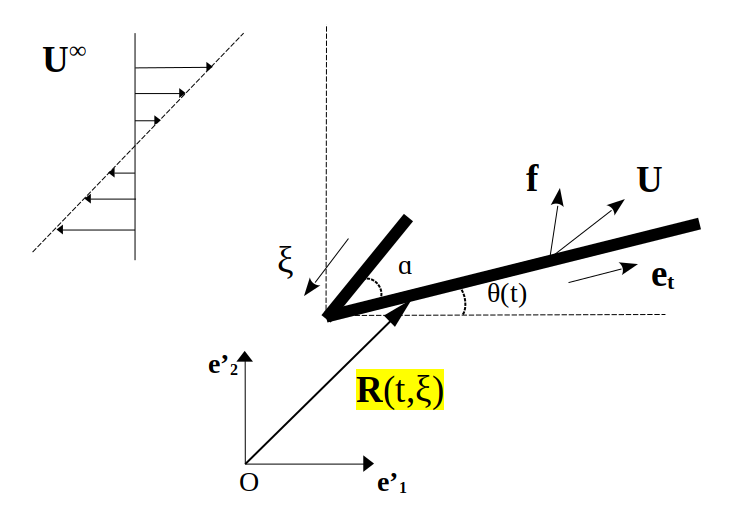
\includegraphics[width=1\textwidth]{plots/rigid_particle2.png}
				\end{center}
				%	\setlength{\abovecaptionskip}{-0.5 cm}
			\end{figure}
			\column{.55\textwidth}
			\small \bi 
			\item \colorbox{yellow}{$\mathbf{R}(t,\xi)$}: particle geometry.
			\item $\mathbf{e}_t$: tangent to the surface of particle.
			\item $\theta(t)$: particle orientation.
			\item $\mathbf{U}^\infty$: velocity of background flow.
			\item $\mathbf{U}$: local $\&$ instantaneous velocity of particle.
			\ei
		\end{columns}\vspace{0.5cm}
	\end{overlayarea}
\end{frame}

%%%%%%%%%%%%%%%%%%%%%%%%%%%%%%%%%%%%%%%%%%%%%%%%%%%%%%%%%%%%%%%%%%%%%%

\begin{frame}
	\frametitle{Theory: slender body theory}
	\begin{overlayarea}{\textwidth}{\textheight}
		\vspace{-0.8cm}
		\begin{columns}
			\column{.6\textwidth}	
			\begin{figure}[htb]
				\begin{center}
					% specify width as 80% of the width of the text on the page
					% we can also specify a width in centimetres, e.g. [width=8cm]
					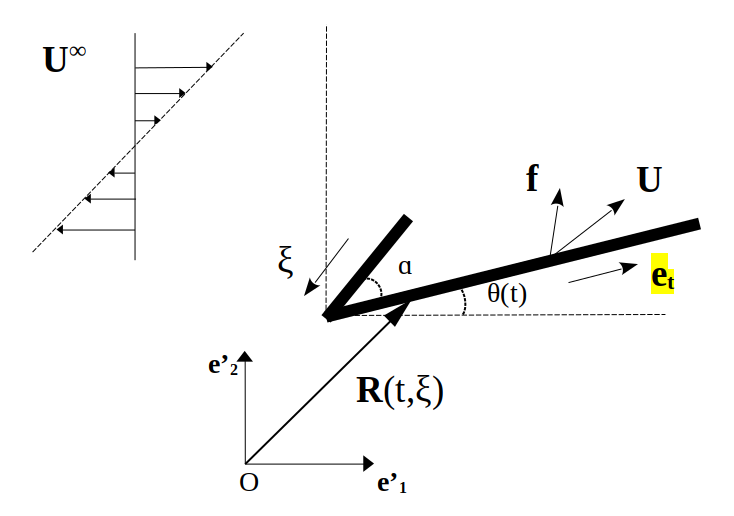
\includegraphics[width=1\textwidth]{plots/rigid_particle3.png}
				\end{center}
				%	\setlength{\abovecaptionskip}{-0.5 cm}
			\end{figure}
			\column{.55\textwidth}
			\small \bi 
			\item $\mathbf{R}(t,\xi)$: particle geometry.
			\item \colorbox{yellow}{$\mathbf{e}_t$}: tangent to the surface of particle.
			\item $\theta(t)$: particle orientation.
			\item $\mathbf{U}^\infty$: velocity of background flow.
			\item $\mathbf{U}$: local $\&$ instantaneous velocity of particle.
			\ei
		\end{columns}\vspace{0.5cm}
	\end{overlayarea}
\end{frame}

%%%%%%%%%%%%%%%%%%%%%%%%%%%%%%%%%%%%%%%%%%%%%%%%%%%%%%%%%%%%%%%%%%%%%%


\begin{frame}
	\frametitle{Theory: slender body theory}
	\begin{overlayarea}{\textwidth}{\textheight}
		\vspace{-0.8cm}
		\begin{columns}
			\column{.6\textwidth}	
			\begin{figure}[htb]
				\begin{center}
					% specify width as 80% of the width of the text on the page
					% we can also specify a width in centimetres, e.g. [width=8cm]
					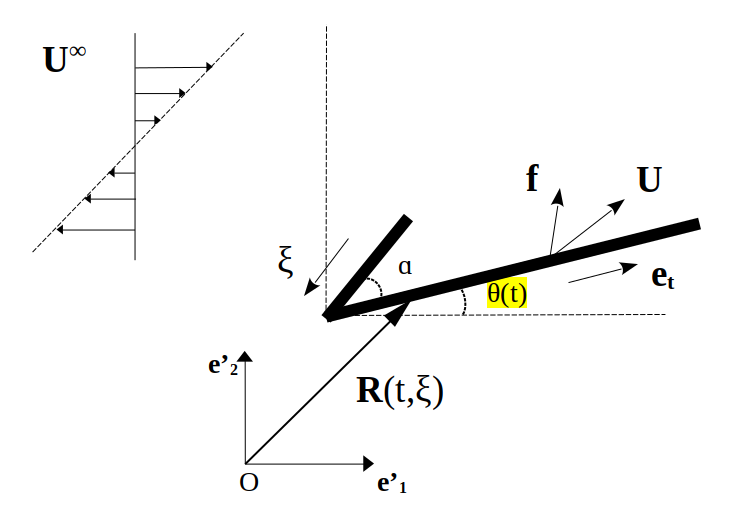
\includegraphics[width=1\textwidth]{plots/rigid_particle4.png}
				\end{center}
				%	\setlength{\abovecaptionskip}{-0.5 cm}
			\end{figure}
			\column{.55\textwidth}
			\small \bi 
			\item $\mathbf{R}(t,\xi)$: particle geometry.
			\item $\mathbf{e}_t$: tangent to the surface of particle.
			\item \colorbox{yellow}{$\theta(t)$}: particle orientation.
			\item $\mathbf{U}^\infty$: velocity of background flow.
			\item $\mathbf{U}$: local $\&$ instantaneous velocity of particle.
			\ei
		\end{columns}\vspace{0.5cm}
	\end{overlayarea}
\end{frame}

%%%%%%%%%%%%%%%%%%%%%%%%%%%%%%%%%%%%%%%%%%%%%%%%%%%%%%%%%%%%%%%%%%%%%%


\begin{frame}
	\frametitle{Theory: slender body theory}
	\begin{overlayarea}{\textwidth}{\textheight}
		\vspace{-0.8cm}
		\begin{columns}
			\column{.6\textwidth}	
			\begin{figure}[htb]
				\begin{center}
					% specify width as 80% of the width of the text on the page
					% we can also specify a width in centimetres, e.g. [width=8cm]
					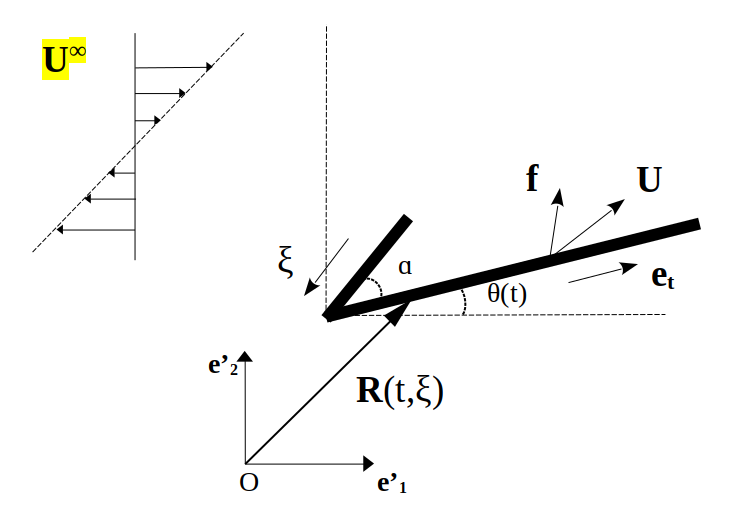
\includegraphics[width=1\textwidth]{plots/rigid_particle5.png}
				\end{center}
				%	\setlength{\abovecaptionskip}{-0.5 cm}
			\end{figure}
			\column{.55\textwidth}
			\small \bi 
			\item $\mathbf{R}(t,\xi)$: particle geometry.
			\item $\mathbf{e}_t$: tangent to the surface of particle.
			\item $\theta(t)$: particle orientation.
			\item \colorbox{yellow}{$\mathbf{U}^\infty$}: velocity of background flow.
			\item $\mathbf{U}$: local $\&$ instantaneous velocity of particle.
			\ei
		\end{columns}\vspace{0.5cm}
	\end{overlayarea}
\end{frame}

%%%%%%%%%%%%%%%%%%%%%%%%%%%%%%%%%%%%%%%%%%%%%%%%%%%%%%%%%%%%%%%%%%%%%%

\begin{frame}
	\frametitle{Theory: slender body theory}
	\begin{overlayarea}{\textwidth}{\textheight}
		\vspace{-0.8cm}
		\begin{columns}
			\column{.6\textwidth}	
			\begin{figure}[htb]
				\begin{center}
					% specify width as 80% of the width of the text on the page
					% we can also specify a width in centimetres, e.g. [width=8cm]
					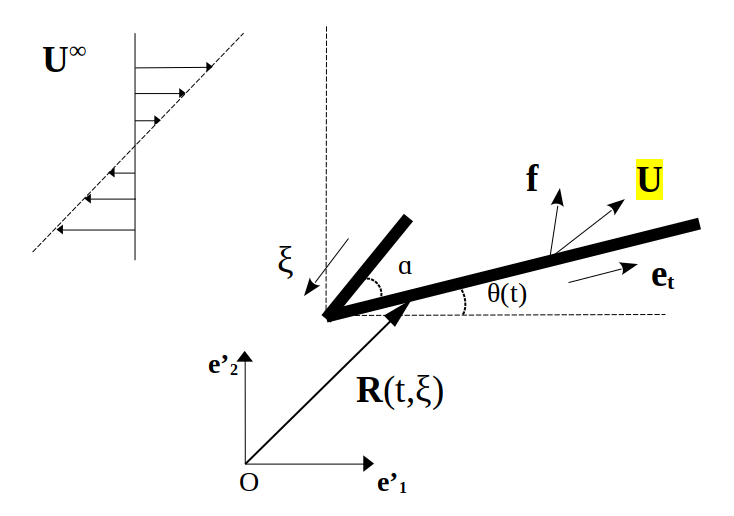
\includegraphics[width=1\textwidth]{plots/rigid_particle6.png}
				\end{center}
				%	\setlength{\abovecaptionskip}{-0.5 cm}
			\end{figure}
			\column{.55\textwidth}
			\small \bi 
			\item $\mathbf{R}(t,\xi)$: particle geometry.
			\item $\mathbf{e}_t$: tangent to the surface of particle.
			\item $\theta(t)$: particle orientation.
			\item $\mathbf{U}^\infty$: velocity of background flow.
			\item \colorbox{yellow}{$\mathbf{U}$}: local $\&$ instantaneous velocity of particle.
			\ei
		\end{columns}\vspace{0.5cm}
	\end{overlayarea}
\end{frame}

%%%%%%%%%%%%%%%%%%%%%%%%%%%%%%%%%%%%%%%%%%%%%%%%%%%%%%%%%%%%%%%%%%%%%%


\begin{frame}
	\frametitle{Theory: slender body theory}
	\begin{overlayarea}{\textwidth}{\textheight}
		\vspace{-0.8cm}
		\begin{columns}
			\column{.6\textwidth}	
			\begin{figure}[htb]
				\begin{center}
					% specify width as 80% of the width of the text on the page
					% we can also specify a width in centimetres, e.g. [width=8cm]
					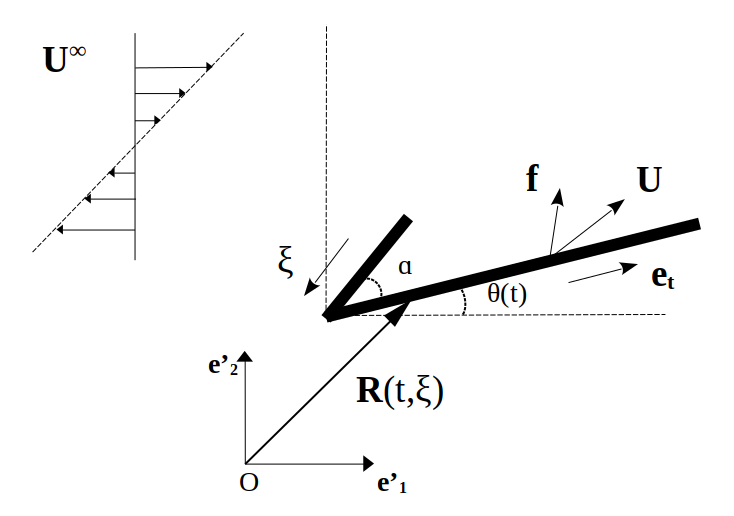
\includegraphics[width=1\textwidth]{plots/rigid_particle7.png}
				\end{center}
				%	\setlength{\abovecaptionskip}{-0.5 cm}
			\end{figure}
			\column{.55\textwidth}
			\small \bi 
			\item $\mathbf{R}(t,\xi)$: particle geometry.
			\item $\mathbf{e}_t$: tangent to the surface of particle.
			\item $\theta(t)$: particle orientation.
			\item $\mathbf{U}^\infty$: velocity of background flow.
			\item $\mathbf{U}$: local $\&$ instantaneous velocity of particle.
			\ei
		\end{columns}\vspace{0.5cm}
		From the slender body theory, the non-dimensional fluid traction is obtained as flows:
		\begin{equation*}
			\mathbf{f}_f=\left(\mathbf{I}-\frac{1}{2}\mathbf{e}_t\mathbf{e}_t\right)\cdot(\mathbf{U}^{\infty}-\mathbf{U}).
		\end{equation*}
	\end{overlayarea}
\end{frame}

%%%%%%%%%%%%%%%%%%%%%%%%%%%%%%%%%%%%%%%%%%%%%%%%%%%%%%%%%%%%%%%%%%%%%%


\begin{frame}
	\frametitle{Theory: slender body theory}
	\begin{overlayarea}{\textwidth}{\textheight}
	\vspace{-1cm}
		\begin{columns}
		\column{.65\textwidth}	
	\begin{figure}[htb]
		\begin{center}
			% specify width as 80% of the width of the text on the page
			% we can also specify a width in centimetres, e.g. [width=8cm]
			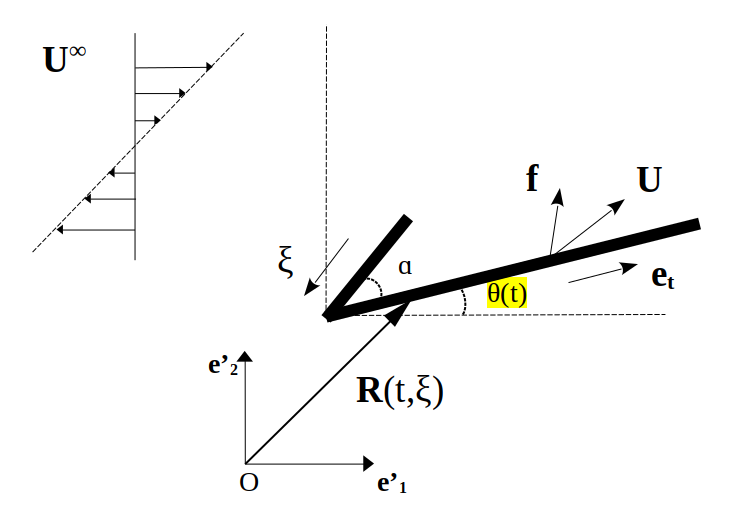
\includegraphics[width=0.8\textwidth]{plots/rigid_particle4.png}
		\end{center}
		%	\setlength{\abovecaptionskip}{-0.5 cm}
	\end{figure}\vspace{0.3cm}
	\column{.5\textwidth}
	  \small From the slender body theory, the non-dimensional fluid traction is obtained as flows:
	\begin{equation*}
		\mathbf{f}_f=\left(\mathbf{I}-\frac{1}{2}\mathbf{e}_t\mathbf{e}_t\right)\cdot(\mathbf{U}^{\infty}-\mathbf{U}).
	\end{equation*}
		\end{columns}\vspace{-0.5cm}
	\begin{columns}
		\column{.58\textwidth}	
	\bi \small
 	\item Net drag and net torque: 	\scriptsize
	\begin{equation*}
		\label{eqn:52}
		\textbf{F}=\int^1_0 \textbf{f}_f\, \left|\frac{\partial\textbf{R}}{\partial\xi}\right|\,d\xi, 
	\end{equation*}
	\begin{equation*}
		\label{eqn:53}
		\mathbf{T}\cdot\textbf{e}_z=\left\{\int^1_0 \left[(\textbf{R}-\textbf{R}_{centre})\times \textbf{f}_f\,\right]\,\left|\frac{\partial\textbf{R}}{\partial\xi}\right|\,d\xi\right\}\cdot\textbf{e}_z,
	\end{equation*}\vspace{-0.3cm}
	where 
	\begin{equation*}
		\textbf{R}_{centre}=\int^1_0 \textbf{R}\,\Big|\frac{\partial\textbf{R}}{\partial\xi}\Big|\,d\xi.
	\end{equation*}
\ei
	\column{.58\textwidth} \vspace{-0.1cm}
	\bi
	\item \small No rotation: \scriptsize
	\begin{equation*}
		\frac{d\theta(t)}{dt}=0.
	\end{equation*}
 \item \small Find equilibrium:
 \scriptsize
	\begin{equation*}
		\left.\begin{aligned}
		\textbf{F}\,(\textbf{R}_0(\xi), V, U_0, \theta_{eq})=\textbf{0}\\
		\{\mathbf{T}\cdot\textbf{e}_z\}\,(\textbf{R}_0(\xi), V, U_0, \theta_{eq})=0\\
		\frac{d\theta(t)}{dt}=0
		\end{aligned}\right\}\Longrightarrow \colorbox{yellow}{$\theta_{eq}$}.
	\end{equation*} 
\ei
\end{columns}
	%\selectfont \fontsize{10}{15}\selectfont
	\end{overlayarea}
\end{frame}

%%%%%%%%%%%%%%%%%%%%%%%%%%%%%%%%%%%%%%%%%%%%%%%%%%%%%%%%%%%%%%%%%%%%%%



\begin{frame}
	\frametitle{Theory: slender body theory}
	\begin{overlayarea}{\textwidth}{\textheight}
		\vspace{-1cm}
		\begin{columns}
			\column{.65\textwidth}	
			\begin{figure}[htb]
				\begin{center}
					% specify width as 80% of the width of the text on the page
					% we can also specify a width in centimetres, e.g. [width=8cm]
					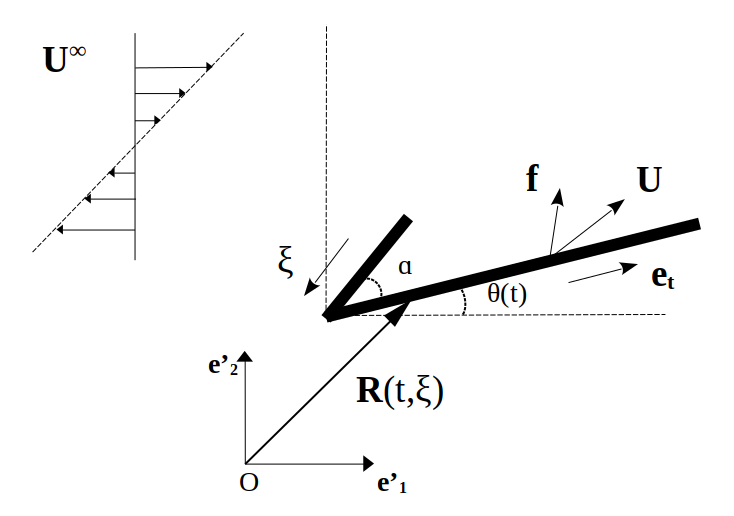
\includegraphics[width=0.8\textwidth]{plots/rigid_particle7.png}
				\end{center}
				%	\setlength{\abovecaptionskip}{-0.5 cm}
			\end{figure}\vspace{0.3cm}
			\column{.5\textwidth}
			\small From the slender body theory, the non-dimensional fluid traction is obtained as flows:
			\begin{equation*}
				\mathbf{f}_f=\left(\mathbf{I}-\frac{1}{2}\mathbf{e}_t\mathbf{e}_t\right)\cdot(\mathbf{U}^{\infty}-\mathbf{U}).
			\end{equation*}
		\end{columns}\vspace{-0.5cm}
	Validation: \vspace{-0.4cm}
		\begin{figure}
		\begin{minipage}{0.46\linewidth}
			\footnotesize Stone's results
			\centering			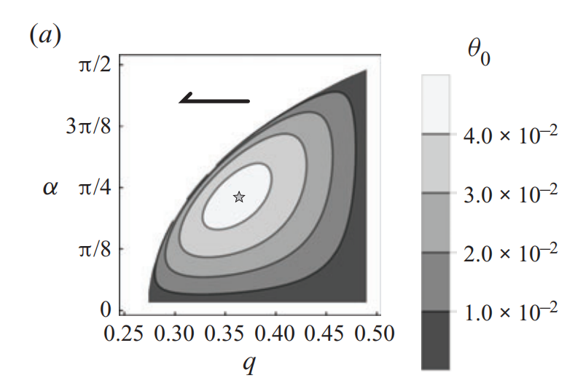
\includegraphics[width=\linewidth]{plots/plot10.png}
		\end{minipage}
		\begin{minipage}{0.52\linewidth}
			\centering
			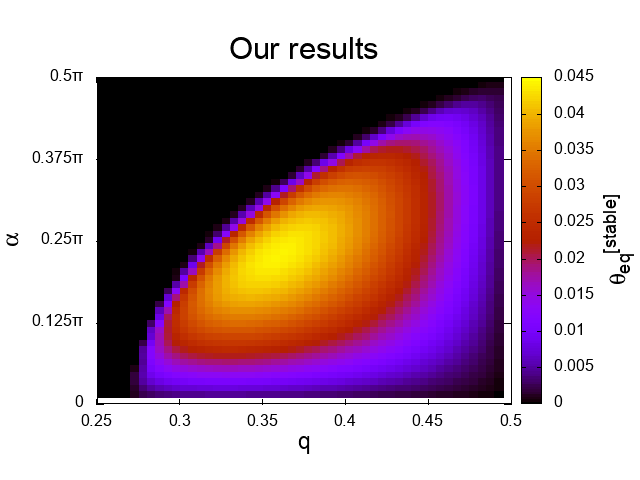
\includegraphics[width=\linewidth]{plots/analytical_straight_contour_theta_range.png} 
		\end{minipage}
	\end{figure}
	\end{overlayarea}
\end{frame}

%%%%%%%%%%%%%%%%%%%%%%%%%%%%%%%%%%%%%%%%%%%%%%%%%%%%%%%%%%%%%%%%%%%%%%



\begin{frame}
	\frametitle{The new bit: elasticity}
	\begin{overlayarea}{\textwidth}{\textheight}
\vspace{-0.5cm}\small	Now, consider elasticity:\vspace{-0.3cm}
		\begin{columns}
		\column{.75\textwidth}	\vspace{-0.5cm}
		\begin{figure}[htb]
			\begin{center}
				% specify width as 80% of the width of the text on the page
				% we can also specify a width in centimetres, e.g. [width=8cm]
				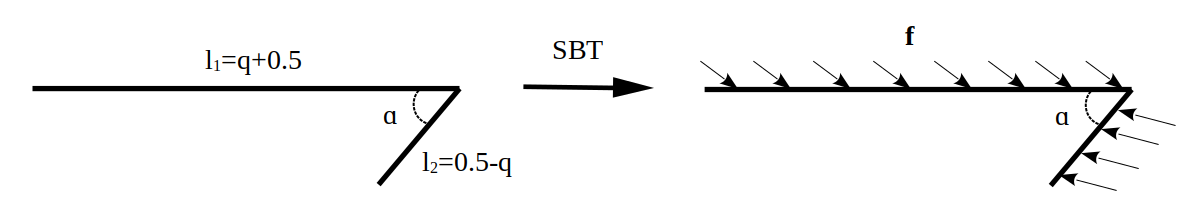
\includegraphics[width=1.05\textwidth]{plots/shape_to_traction.png}
			\end{center}
			%	\setlength{\abovecaptionskip}{-0.5 cm}
		\end{figure}
		\column{.4\textwidth}
		\bi 
		\item \small So far, SBT:
		
		 shape $\Longrightarrow$ traction $\mathbf{f}_f$.
		\ei
	\end{columns}
	\end{overlayarea}
\end{frame}

%%%%%%%%%%%%%%%%%%%%%%%%%%%%%%%%%%%%%%%%%%%%%%%%%%%%%%%%%%%%%%%%%%%%%%

\begin{frame}
	\frametitle{The new bit: elasticity}
	\begin{overlayarea}{\textwidth}{\textheight}
		\vspace{-0.5cm}\small	Now, consider elasticity:\vspace{-0.3cm}
		\begin{columns}
			\column{.75\textwidth}	\vspace{-0.5cm}
			\begin{figure}[htb]
				\begin{center}
					% specify width as 80% of the width of the text on the page
					% we can also specify a width in centimetres, e.g. [width=8cm]
					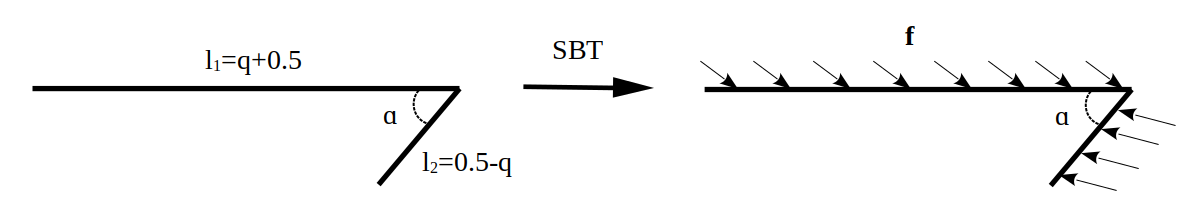
\includegraphics[width=1.05\textwidth]{plots/shape_to_traction.png}
				\end{center}
				%	\setlength{\abovecaptionskip}{-0.5 cm}
			\end{figure}
			\column{.4\textwidth}
			\bi 
			\item \small So far, SBT:
			
			shape $\Longrightarrow$ traction $\mathbf{f}_f$.
			\ei
		\end{columns}
		\begin{columns}
			\column{.75\textwidth}	\vspace{-1cm}
			\begin{figure}[htb]
				\begin{center}
					% specify width as 80% of the width of the text on the page
					% we can also specify a width in centimetres, e.g. [width=8cm]
					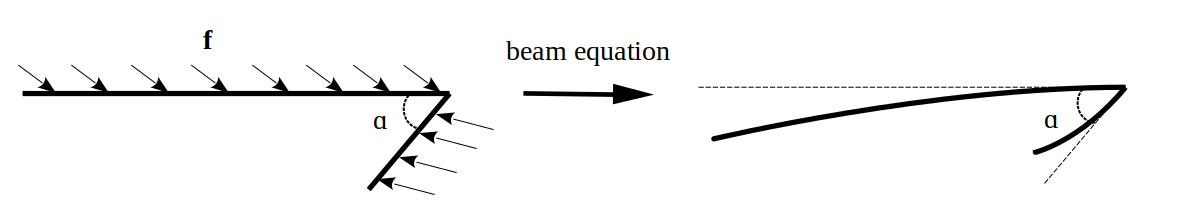
\includegraphics[width=1.05\textwidth]{plots/traction_to_shape.png}
				\end{center}
				%	\setlength{\abovecaptionskip}{-0.5 cm}
			\end{figure}
			\column{.4\textwidth}\vspace{-0.1cm}
			\bi 
			\item \small Now, beam equation:
			
			traction $\mathbf{f}_s$ $\Longrightarrow$ shape.
			\ei
		\end{columns}\vspace{0.2cm}
	\end{overlayarea}
\end{frame}

%%%%%%%%%%%%%%%%%%%%%%%%%%%%%%%%%%%%%%%%%%%%%%%%%%%%%%%%%%%%%%%%%%%%%%

\begin{frame}
	\frametitle{The new bit: elasticity}
	\begin{overlayarea}{\textwidth}{\textheight}
		\vspace{-0.5cm}\small	Now, consider elasticity:\vspace{-0.3cm}
		\begin{columns}
			\column{.75\textwidth}	\vspace{-0.5cm}
			\begin{figure}[htb]
				\begin{center}
					% specify width as 80% of the width of the text on the page
					% we can also specify a width in centimetres, e.g. [width=8cm]
					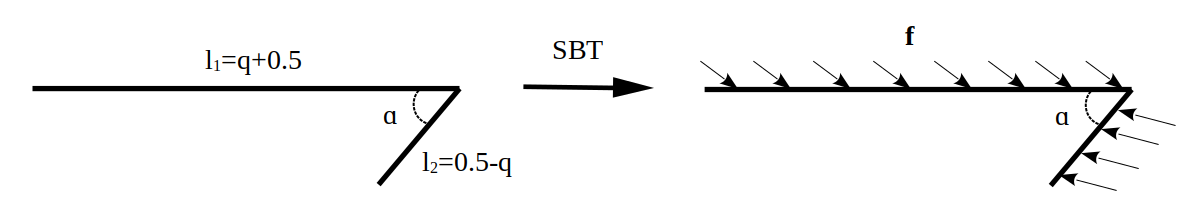
\includegraphics[width=1.05\textwidth]{plots/shape_to_traction.png}
				\end{center}
				%	\setlength{\abovecaptionskip}{-0.5 cm}
			\end{figure}
			\column{.4\textwidth}
			\bi 
			\item \small So far, SBT:
			
			shape $\Longrightarrow$ traction $\mathbf{f}_f$.
			\ei
		\end{columns}
		\begin{columns}
			\column{.75\textwidth}	\vspace{-1cm}
			\begin{figure}[htb]
				\begin{center}
					% specify width as 80% of the width of the text on the page
					% we can also specify a width in centimetres, e.g. [width=8cm]
					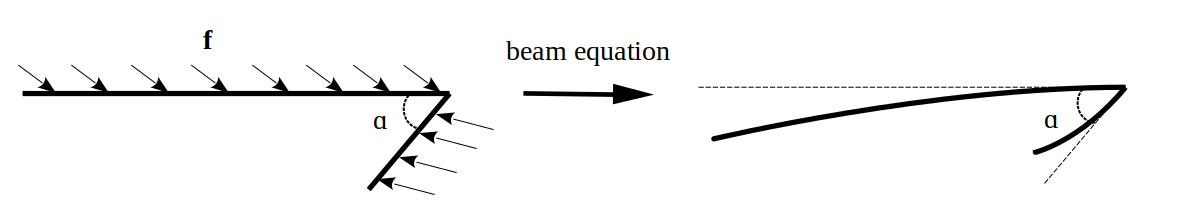
\includegraphics[width=1.05\textwidth]{plots/traction_to_shape.png}
				\end{center}
				%	\setlength{\abovecaptionskip}{-0.5 cm}
			\end{figure}
			\column{.4\textwidth}\vspace{-0.1cm}
			\bi 
			\item \small Now, beam equation:
			
			traction $\mathbf{f}_s$ $\Longrightarrow$ shape.
			\ei
		\end{columns}\vspace{0.2cm}
		\begin{columns}
			\column{.4\textwidth}	\vspace{-0.6cm} 
			\bi
			\item Fluid-solid interaction: 
			\ei
			\column{.65\textwidth} \vspace{-0.35cm}
			\begin{figure}[htb]
				\begin{center}
					% specify width as 80% of the width of the text on the page
					% we can also specify a width in centimetres, e.g. [width=8cm]
					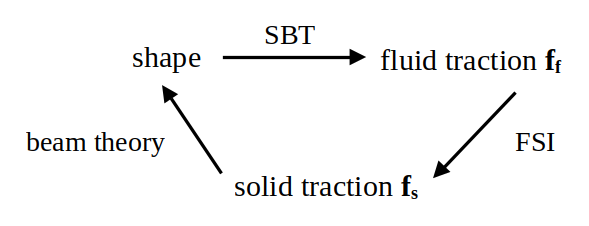
\includegraphics[width=0.9\textwidth]{plots/logic.png}
				\end{center}
				%	\setlength{\abovecaptionskip}{-0.5 cm}
			\end{figure}
		\end{columns}\vspace{0.1cm}
	\end{overlayarea}
\end{frame}

%%%%%%%%%%%%%%%%%%%%%%%%%%%%%%%%%%%%%%%%%%%%%%%%%%%%%%%%%%%%%%%%%%%%%%


\begin{frame}
	\frametitle{The new bit: elasticity}
	\begin{overlayarea}{\textwidth}{\textheight}
		\vspace{-0.5cm}\small	Now, consider elasticity:\vspace{-0.3cm}
		\begin{columns}
			\column{.75\textwidth}	\vspace{-0.5cm}
			\begin{figure}[htb]
				\begin{center}
					% specify width as 80% of the width of the text on the page
					% we can also specify a width in centimetres, e.g. [width=8cm]
					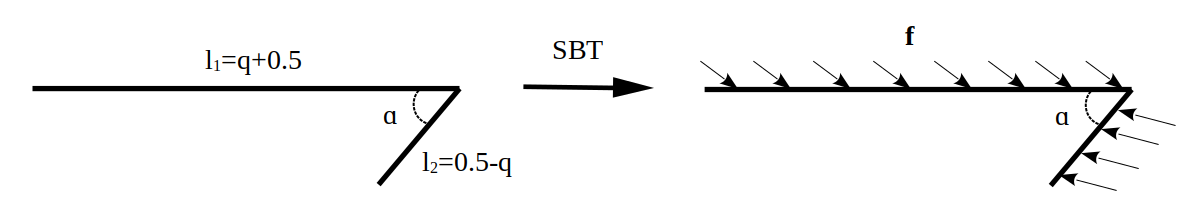
\includegraphics[width=1.05\textwidth]{plots/shape_to_traction.png}
				\end{center}
				%	\setlength{\abovecaptionskip}{-0.5 cm}
			\end{figure}
			\column{.4\textwidth}
			\bi 
			\item \small So far, SBT:
			
			shape $\Longrightarrow$ traction $\mathbf{f}_f$.
			\ei
		\end{columns}
		\begin{columns}
			\column{.75\textwidth}	\vspace{-1cm}
			\begin{figure}[htb]
				\begin{center}
					% specify width as 80% of the width of the text on the page
					% we can also specify a width in centimetres, e.g. [width=8cm]
					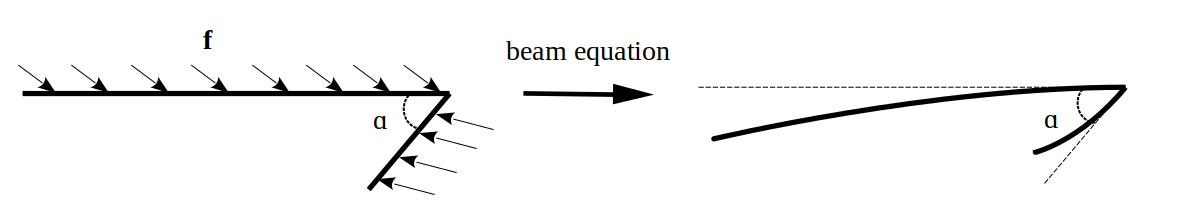
\includegraphics[width=1.05\textwidth]{plots/traction_to_shape.png}
				\end{center}
				%	\setlength{\abovecaptionskip}{-0.5 cm}
			\end{figure}
			\column{.4\textwidth}\vspace{-0.1cm}
			\bi 
			\item \small Now, beam equation:
			
			traction $\mathbf{f}_s$ $\Longrightarrow$ shape.
			\ei
		\end{columns}\vspace{0.2cm}
		\begin{columns}
			\column{.4\textwidth}	\vspace{-0.6cm} 
			\bi
			\item Fluid-solid interaction: 
			\ei
			\column{.65\textwidth} \vspace{-0.35cm}
			\begin{figure}[htb]
				\begin{center}
					% specify width as 80% of the width of the text on the page
					% we can also specify a width in centimetres, e.g. [width=8cm]
					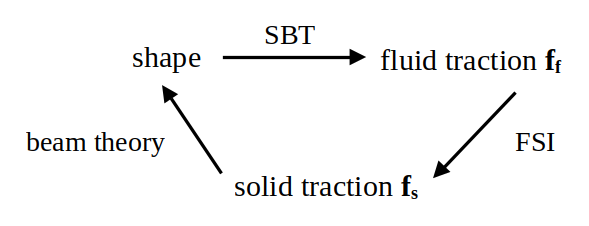
\includegraphics[width=0.9\textwidth]{plots/logic.png}
				\end{center}
				%	\setlength{\abovecaptionskip}{-0.5 cm}
			\end{figure}
		\end{columns}\vspace{0.1cm}
		\bi 
		\item \small Kirchhoff-Love beam theory (\texttt{oomph-lib}):
		\vspace{-0.1cm} \footnotesize 
		\begin{equation*}
			\int_0^1 \Bigg[ (\sigma_0 + \gamma)\, \delta \gamma 
			+ \frac{1}{12} h^2 \kappa\, \delta \kappa \Bigg. 
			\Bigg. - \frac{1}{h} \sqrt{\frac{A}{a}}\, \textbf{f}_s \cdot \delta \textbf{R}_0 \Bigg] \sqrt{a}\, d\xi = 0.
		\end{equation*}
		\ei 
	\end{overlayarea}
\end{frame}

%%%%%%%%%%%%%%%%%%%%%%%%%%%%%%%%%%%%%%%%%%%%%%%%%%%%%%%%%%%%%%%%%%%%%%



\begin{frame}
	\frametitle{Fluid-solid interaction}
	\begin{overlayarea}{\textwidth}{\textheight}
	\small Note: equations shown were nondimensionalized on their natural scales:
	\begin{equation*}
		\label{eqn:102}
		\mathbf{f}^*=c_\perp\,\mathcal{L}\,\dot{\gamma}\,\mathbf{f}_{f}=K\,\mathbf{f}_{s}.
	\end{equation*}
	$c_\perp$ drag coefficient. 
	\begin{equation*}
		\textbf{f}_{s}=\frac{c_\perp\,\mathcal{L}\,\dot{\gamma}}{K}\,\textbf{f}_{f}.
	\end{equation*}

	FSI parameter: 
	\begin{equation*}
		\label{eqn:38}
		\mathcal{I}=\frac{c_\perp\,\mathcal{L}\,\dot{\gamma}}{K}=\frac{\text{"fluid stress"}}{\text{"bending stiffness"}}.
	\end{equation*}
		\begin{columns}
			\column{.35\textwidth}	
			  \small \bi
			 \item $\mathcal{I}=0$: rigid;
			 \item $\mathcal{I}>0$: elastic.
			 \ei
			\column{.65\textwidth} \vspace{-0.8cm}	
		\end{columns}
	\end{overlayarea}
\end{frame}



%%%%%%%%%%%%%%%%%%%%%%%%%%%%%%%%%%%%%%%%%%%%%%%%%%%%%%%%%%%%%%%%%%%%%%



\begin{frame}
	\frametitle{Summary}
	\begin{overlayarea}{\textwidth}{\textheight}
		\vspace{-0.3cm}	
	\begin{itemize}
		\item Elastic (initial configuration):
		\begin{figure}[htb]
			\begin{center}
				% specify width as 80% of the width of the text on the page
				% we can also specify a width in centimetres, e.g. [width=8cm]
				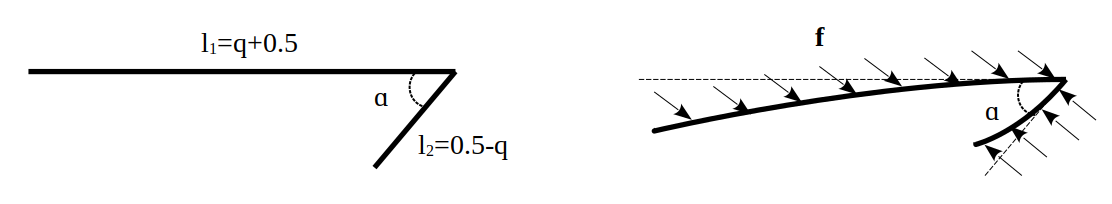
\includegraphics[width=0.85\textwidth]{plots/geometry.png}
			\end{center}
			%	\setlength{\abovecaptionskip}{-0.5 cm}
		\end{figure}\vspace{0.1cm}	
	\item Equations: \small
		$\quad \quad\quad
	\left.	\begin{aligned}
			\text{beam equation}\\
			\text{slender body theory}\\
			\text{drag-free}\\
			\text{torque-free}\\
			\text{no rotation}
		\end{aligned}\right\}\Longrightarrow \theta_{eq}, \mathbf{R}.
	$\vspace{-0.75cm}	
		\begin{columns}
		\column{.5\textwidth}	
	\begin{figure}[htb]
		\begin{center}
			% specify width as 80% of the width of the text on the page
			% we can also specify a width in centimetres, e.g. [width=8cm]
			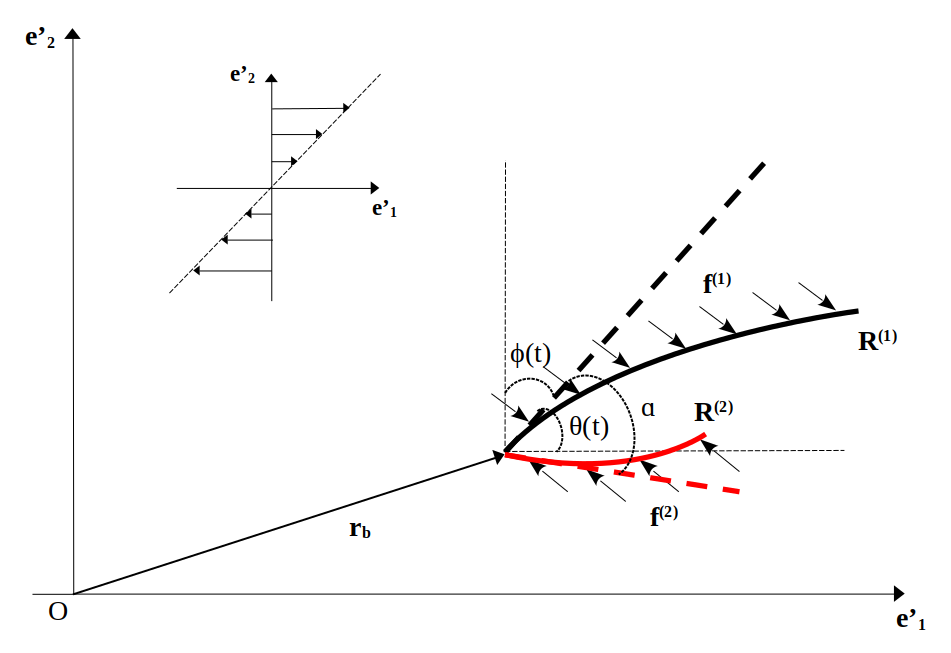
\includegraphics[width=0.95\textwidth]{plots/fluid.png}
		\end{center}
		%	\setlength{\abovecaptionskip}{-0.5 cm}
	\end{figure}
		\column{.5\textwidth} 
	\end{columns}
	\end{itemize}
	\end{overlayarea}
\end{frame}

%%%%%%%%%%%%%%%%%%%%%%%%%%%%%%%%%%%%%%%%%%%%%%%%%%%%%%%%%%%%%%%%%%%%%%

\begin{frame}
	\frametitle{Reminder}
	\begin{overlayarea}{\textwidth}{\textheight}
	\vspace{0.5cm}	
	Fixed points: \small of four fixed orientations, two differ from the other two by an angle of $\pi$.\vspace{0.5cm}	
	\begin{itemize} 
		\item Rigid:
		\begin{figure}[htb]
			\begin{center}
				% specify width as 80% of the width of the text on the page
				% we can also specify a width in centimetres, e.g. [width=8cm]
				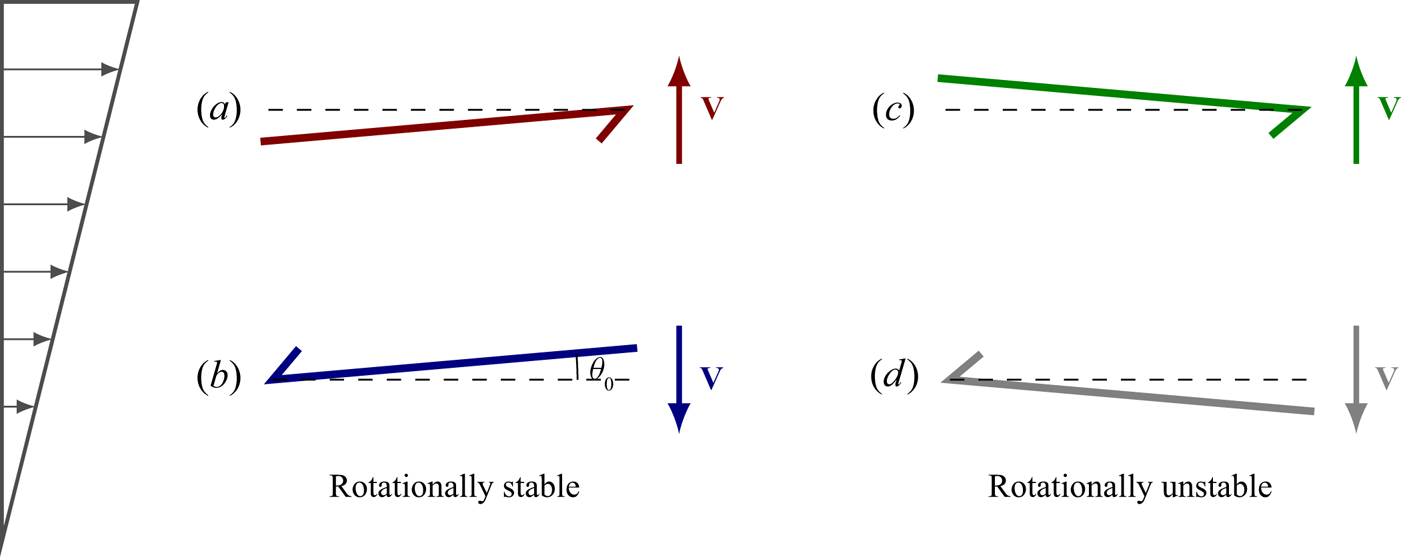
\includegraphics[width=0.6\textwidth]{plots/stone3.png}
			\end{center}
			%	\setlength{\abovecaptionskip}{-0.5 cm}
		\end{figure}
		\item Elastic: same structure.
	\end{itemize}
	\end{overlayarea}
\end{frame}

%%%%%%%%%%%%%%%%%%%%%%%%%%%%%%%%%%%%%%%%%%%%%%%%%%%%%%%%%%%%%%%%%%%%%%


\frame[plain]{\frametitle{Results: effect of increasing $\mathcal{I}$}
	\begin{overlayarea}{\textwidth}{\textheight}\vspace{-0.3cm}
		\foreach \index in {1,...,1} % 210}
	{\pgfmathsetmacro\picnumber{int(\index-1)}	
		\only<\index>{% FRAME: \index  \ \picnumber	
			\begin{center}	
				\includegraphics<\index>[width=0.9\textwidth]{plots/combine_elastic_beam_I_theta_q_0.40_alpha_0.230pi_initial_-4.80_\picnumber.png}	
			\end{center}              	
			%\includegraphics<\index>[width=2\textwidth]{images/warped_disk/fe_soln/resized/frame\picnumber.png}}
		\vspace{-0.3cm}
		\bi
	\item $\mathcal{I}=0$: two known solutions.
	\item Ratio: shape plots are not $1:1$.
	\ei
	}
	%\scalebox{1.0}{\import{\PaperImagePath}{trajectories_Rc=0.5_red_karaoke/frame1.tex}}
}
\end{overlayarea}
}


%%%%%%%%%%%%%%%%%%%%%%%%%%%%%%%%%%%%%%%%%%%%%%%%%%%%%%%%%%%%%%%%%%%%%%


\frame[plain]{\frametitle{Results: effect of increasing $\mathcal{I}$}
	\begin{overlayarea}{\textwidth}{\textheight}\vspace{-0.3cm}
		\foreach \index in {1,...,1} % 210}
	{\pgfmathsetmacro\picnumber{int(\index)}	
		\only<\index>{% FRAME: \index  \ \picnumber	
			\begin{center}	
				\includegraphics<\index>[width=0.9\textwidth]{plots/combine_elastic_beam_I_theta_q_0.40_alpha_0.230pi_initial_-4.80_\picnumber.png}	
			\end{center}              	
			%\includegraphics<\index>[width=2\textwidth]{images/warped_disk/fe_soln/resized/frame\picnumber.png}}
		\vspace{-0.3cm}
			\bi
		\item Evolve $\theta_{eq}$ for $\mathcal{I}>0$.
		\ei
	}
	%\scalebox{1.0}{\import{\PaperImagePath}{trajectories_Rc=0.5_red_karaoke/frame1.tex}}
}
\end{overlayarea}
}


%%%%%%%%%%%%%%%%%%%%%%%%%%%%%%%%%%%%%%%%%%%%%%%%%%%%%%%%%%%%%%%%%%%%%%


\frame[plain]{\frametitle{Results: effect of increasing $\mathcal{I}$}
	\begin{overlayarea}{\textwidth}{\textheight}\vspace{-0.3cm}
		\foreach \index in {1,...,7} % 210}
	{\pgfmathsetmacro\picnumber{int(\index+1)}	
		\only<\index>{% FRAME: \index  \ \picnumber	
			\begin{center}	
			\includegraphics<\index>[width=0.9\textwidth]{plots/combine_elastic_beam_I_theta_q_0.40_alpha_0.230pi_initial_-4.80_\picnumber.png}	
			\end{center}              	
			%\includegraphics<\index>[width=2\textwidth]{images/warped_disk/fe_soln/resized/frame\picnumber.png}}
		    \vspace{-0.3cm}
			\bi
	     	\item Upper branch: particles deform $\&$ rotate.
		    \ei	
	}
	%\scalebox{1.0}{\import{\PaperImagePath}{trajectories_Rc=0.5_red_karaoke/frame1.tex}}
}
\end{overlayarea}
}

\frame[plain]{\frametitle{Results: effect of increasing $\mathcal{I}$}
	\begin{overlayarea}{\textwidth}{\textheight}\vspace{-0.3cm}
		\foreach \index in {1,...,6} % 210}
	{\pgfmathsetmacro\picnumber{int(\index+8)}	
		\only<\index>{% FRAME: \index  \ \picnumber	
			\begin{center}	
				\includegraphics<\index>[width=0.9\textwidth]{plots/combine_elastic_beam_I_theta_q_0.40_alpha_0.230pi_initial_-4.80_\picnumber.png}	
			\end{center}              	
			%\includegraphics<\index>[width=2\textwidth]{images/warped_disk/fe_soln/resized/frame\picnumber.png}}
		\vspace{-0.3cm}
		\bi
		\item Upper branch: particles deform $\&$ rotate.
		\item Lower branch: particles deform $\&$ rotate, too.
		\ei	
	}
	%\scalebox{1.0}{\import{\PaperImagePath}{trajectories_Rc=0.5_red_karaoke/frame1.tex}}
}
\end{overlayarea}
}

%%%%%%%%%%%%%%%%%%%%%%%%%%%%%%%%%%%%%%%%%%%%%%%%%%%%%%%%%%%%%%%%%%%%%%

\frame[plain]{\frametitle{Results: effect of increasing $\mathcal{I}$}
	\begin{overlayarea}{\textwidth}{\textheight}\vspace{-0.3cm}
		\foreach \index in {1,...,1} % 210}
	{\pgfmathsetmacro\picnumber{int(\index+14)}	
		\only<\index>{% FRAME: \index  \ \picnumber	
			\begin{center}	
				\includegraphics<\index>[width=0.9\textwidth]{plots/combine_elastic_beam_I_theta_q_0.40_alpha_0.230pi_initial_-4.80_\picnumber.png}	
			\end{center}              	
			%\includegraphics<\index>[width=2\textwidth]{images/warped_disk/fe_soln/resized/frame\picnumber.png}}
		\vspace{-0.3cm}
		\bi
\item Two branches coalesce in limit point.
\item No solutions for larger $\mathcal{I}$.
\ei
	}
	%\scalebox{1.0}{\import{\PaperImagePath}{trajectories_Rc=0.5_red_karaoke/frame1.tex}}
}
\end{overlayarea}
}


%%%%%%%%%%%%%%%%%%%%%%%%%%%%%%%%%%%%%%%%%%%%%%%%%%%%%%%%%%%%%%%%%%%%%%


\frame[plain]{\frametitle{Results: effect of increasing $\mathcal{I}$}
	\begin{overlayarea}{\textwidth}{\textheight}\vspace{-0.3cm}
		\foreach \index in {1,...,25} % 210}
	{\pgfmathsetmacro\picnumber{int(\index-1)}	
		\only<\index>{% FRAME: \index  \ \picnumber	
			\begin{center}	
				\includegraphics<\index>[width=0.9\textwidth]{plots/initial_combine_elastic_beam_I_theta_q_0.400_alpha_0.180pi_initial_-4.80_\picnumber.png}	
			\end{center}              	
			%\includegraphics<\index>[width=2\textwidth]{images/warped_disk/fe_soln/resized/frame\picnumber.png}}
				\vspace{-0.3cm}
		\bi
		\item Smaller $\alpha$.
		\item Again start with two known rigid solutions.
		\ei	
	}
	%\scalebox{1.0}{\import{\PaperImagePath}{trajectories_Rc=0.5_red_karaoke/frame1.tex}}	
}
\end{overlayarea}
}

%%%%%%%%%%%%%%%%%%%%%%%%%%%%%%%%%%%%%%%%%%%%%%%%%%%%%%%%%%%%%%%%%%%%%%


\begin{frame}
	\frametitle{What actually happens?}
	\begin{overlayarea}{\textwidth}{\textheight}\vspace{-0.5cm}
		\foreach \index in {1,...,4} % 210}
	{\pgfmathsetmacro\picnumber{int(\index-1)}	
		\only<\index>{% FRAME: \index  \ \picnumber	
			\begin{center}	
				\includegraphics<\index>[width=0.65\textwidth]{plots/elastic_beam_I_theta_q_0.400_alpha_\picnumber.png}	
			\end{center}              	
			%\includegraphics<\index>[width=2\textwidth]{images/warped_disk/fe_soln/resized/frame\picnumber.png}}
		\vspace{-0.4cm}
		\bi\small
		\item First case: red line only.
		\ei	
	}
	%\scalebox{1.0}{\import{\PaperImagePath}{trajectories_Rc=0.5_red_karaoke/frame1.tex}}	
}
\end{overlayarea}
\end{frame}

%%%%%%%%%%%%%%%%%%%%%%%%%%%%%%%%%%%%%%%%%%%%%%%%%%%%%%%%%%%%%%%%%%%%%%


\begin{frame}
	\frametitle{What actually happens?}
	\begin{overlayarea}{\textwidth}{\textheight}\vspace{-0.5cm}
	\foreach \index in {1,...,3} % 210}
{\pgfmathsetmacro\picnumber{int(\index+3)}	
	\only<\index>{% FRAME: \index  \ \picnumber	
		\begin{center}	
			\includegraphics<\index>[width=0.65\textwidth]{plots/elastic_beam_I_theta_q_0.400_alpha_\picnumber.png}	
		\end{center}              	
		%\includegraphics<\index>[width=2\textwidth]{images/warped_disk/fe_soln/resized/frame\picnumber.png}}
	\vspace{-0.4cm}
	\bi\small
	\item First case: red line only.
	\item Second case: variation in $\alpha$ creates disconnected loop (blue).
	\ei	
}
%\scalebox{1.0}{\import{\PaperImagePath}{trajectories_Rc=0.5_red_karaoke/frame1.tex}}	
}
\end{overlayarea}
\end{frame}

%%%%%%%%%%%%%%%%%%%%%%%%%%%%%%%%%%%%%%%%%%%%%%%%%%%%%%%%%%%%%%%%%%%%%%


\begin{frame}
	\frametitle{What actually happens?}
	\begin{overlayarea}{\textwidth}{\textheight}\vspace{-0.5cm}
		\begin{figure}[htb]
		\begin{center}
			% specify width as 80% of the width of the text on the page
			% we can also specify a width in centimetres, e.g. [width=8cm]
			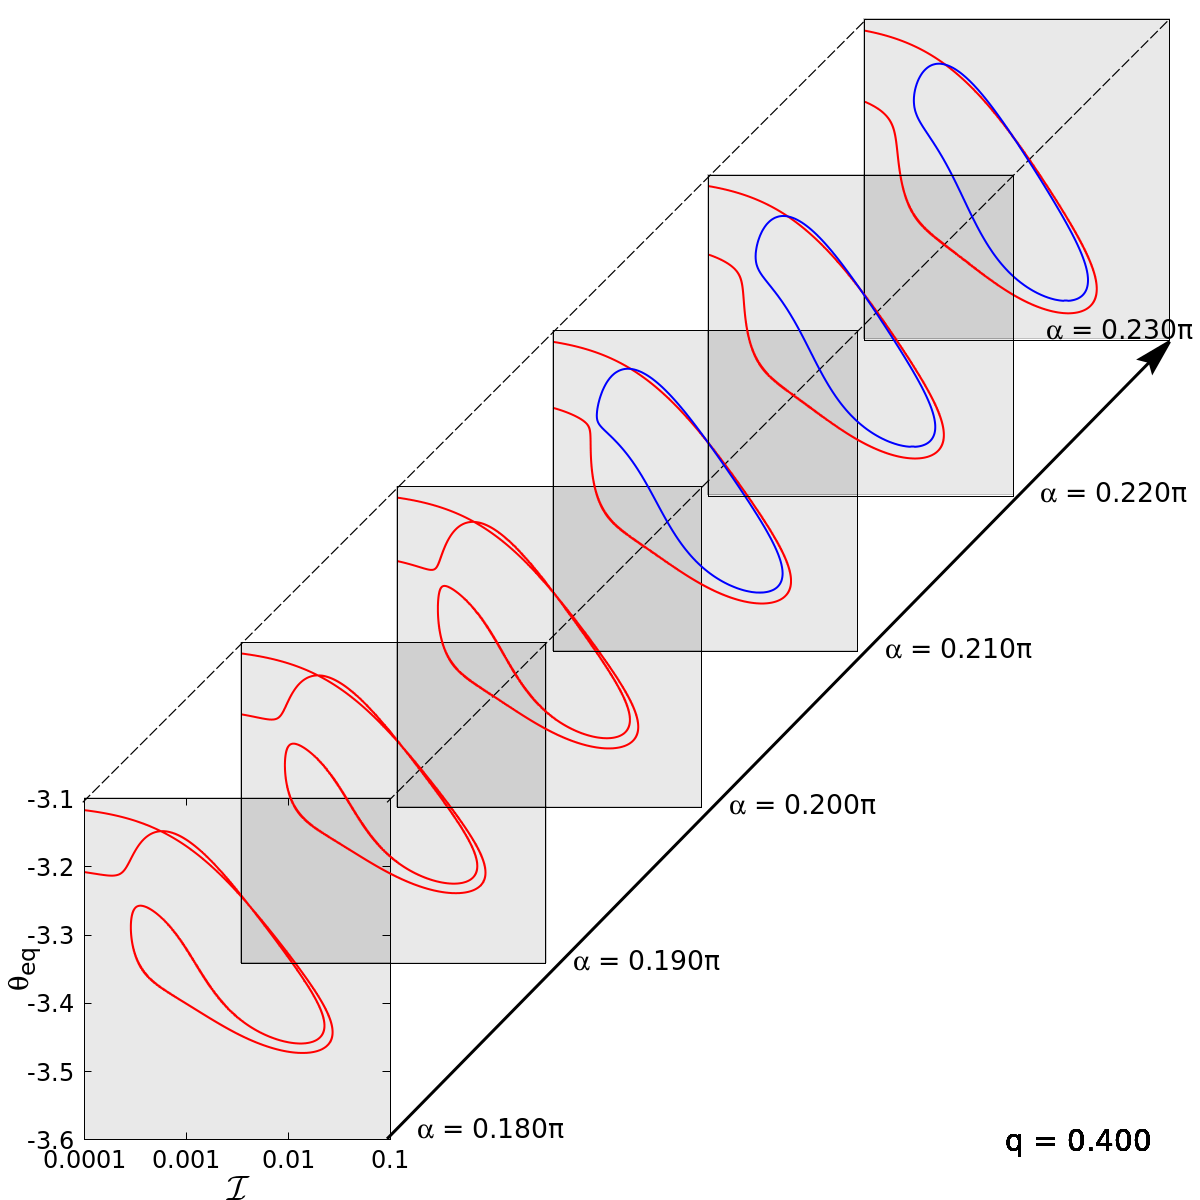
\includegraphics[width=0.65\textwidth]{plots/elastic_beam_I_theta_q_0.400_alpha_6.png}
		\end{center}
		%	\setlength{\abovecaptionskip}{-0.5 cm}
	\end{figure}\vspace{-7.5cm}
    \begin{figure}[htb]
    	    \raggedright
    		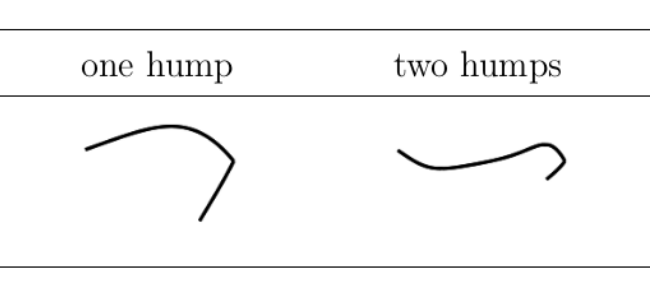
\includegraphics[width=0.4\textwidth]{plots/two_deformations.png}
    	%	\setlength{\abovecaptionskip}{-0.5 cm}
    \end{figure}\vspace{4.6cm}
\bi
\item Second case: red line ("one hump"), blue loop ("two humps"). 
\ei
\end{overlayarea}
\end{frame}

%%%%%%%%%%%%%%%%%%%%%%%%%%%%%%%%%%%%%%%%%%%%%%%%%%%%%%%%%%%%%%%%%%%%%%


\frame[plain]{\frametitle{Stability}
	\begin{overlayarea}{\textwidth}{\textheight}\vspace{-0.3cm}
		\foreach \index in {1,...,1} % 210}
	{\pgfmathsetmacro\picnumber{int(\index+13)}	
		\only<\index>{% FRAME: \index  \ \picnumber	
			\begin{center}	
				\includegraphics<\index>[width=0.9\textwidth]{plots/combine_elastic_beam_I_theta_q_0.40_alpha_0.230pi_initial_-4.80_\picnumber.png}	
			\end{center}              	
			%\includegraphics<\index>[width=2\textwidth]{images/warped_disk/fe_soln/resized/frame\picnumber.png}}
		\vspace{-0.3cm}
		\bi
		\item Speculation:
		
		upper branch: stable,
        lower branch: unstable.
		\ei	
	}
	%\scalebox{1.0}{\import{\PaperImagePath}{trajectories_Rc=0.5_red_karaoke/frame1.tex}}
}
\end{overlayarea}
}

%%%%%%%%%%%%%%%%%%%%%%%%%%%%%%%%%%%%%%%%%%%%%%%%%%%%%%%%%%%%%%%%%%%%%%

\begin{frame}
	\frametitle{Animations (time stepping)}
	\begin{overlayarea}{\textwidth}{\textheight}
		Upper branch:
		\foreach \index in {1,...,133} % 210}
	{\pgfmathsetmacro\picnumber{int(\index-1)}	
		\only<\index>{% FRAME: \index  \ \picnumber	
			\begin{center}	
				\includegraphics<\index>[width=1\textwidth]{plots/plots_for_animation_q_0.40_alpha_41.400_stable/plot_\picnumber.png}	
			\end{center}              	
			%\includegraphics<\index>[width=2\textwidth]{images/warped_disk/fe_soln/resized/frame\picnumber.png}}
		%\vspace{-0.4cm}
		\bi\small
		\item Give a small perturbation.
		\item Should be stable.
		\ei	
	}
	%\scalebox{1.0}{\import{\PaperImagePath}{trajectories_Rc=0.5_red_karaoke/frame1.tex}}	
}
\end{overlayarea}
\end{frame}

%%%%%%%%%%%%%%%%%%%%%%%%%%%%%%%%%%%%%%%%%%%%%%%%%%%%%%%%%%%%%%%%%%%%%%


\begin{frame}
	\frametitle{Animations (time stepping)}
	\begin{overlayarea}{\textwidth}{\textheight}
		Lower branch:
		\foreach \index in {1,...,84} % 210}
	{\pgfmathsetmacro\picnumber{int(\index-1)}	
		\only<\index>{% FRAME: \index  \ \picnumber	
			\begin{center}	
				\includegraphics<\index>[width=1\textwidth]{plots/plots_for_animation_q_0.40_alpha_41.400_unstable/plot_\picnumber.png}	
			\end{center}              	
			%\includegraphics<\index>[width=2\textwidth]{images/warped_disk/fe_soln/resized/frame\picnumber.png}}
		%\vspace{-0.4cm}
		\bi\small
		\item Give a small perturbation.
		\item Should be unstable.
		\ei	
	}
	%\scalebox{1.0}{\import{\PaperImagePath}{trajectories_Rc=0.5_red_karaoke/frame1.tex}}	
}
\end{overlayarea}
\end{frame}

%%%%%%%%%%%%%%%%%%%%%%%%%%%%%%%%%%%%%%%%%%%%%%%%%%%%%%%%%%%%%%%%%%%%%%


\frame[plain]{\frametitle{Stability (smaller $\alpha$)}
	\begin{overlayarea}{\textwidth}{\textheight}\vspace{-0.3cm}
		\foreach \index in {1,...,1} % 210}
	{\pgfmathsetmacro\picnumber{int(\index+22)}	
		\only<\index>{% FRAME: \index  \ \picnumber	
			\begin{center}	
				\includegraphics<\index>[width=0.9\textwidth]{plots/initial_combine_elastic_beam_I_theta_q_0.400_alpha_0.180pi_initial_-4.80_\picnumber.png}	
			\end{center}              	
			%\includegraphics<\index>[width=2\textwidth]{images/warped_disk/fe_soln/resized/frame\picnumber.png}}
		\vspace{-0.3cm}
		\bi
		\item 3 limit points.
		\item Stability of one branch is different from our speculation.
		\ei	
	}
	%\scalebox{1.0}{\import{\PaperImagePath}{trajectories_Rc=0.5_red_karaoke/frame1.tex}}	
}
\end{overlayarea}
}

%%%%%%%%%%%%%%%%%%%%%%%%%%%%%%%%%%%%%%%%%%%%%%%%%%%%%%%%%%%%%%%%%%%%%%

\begin{frame}
	\frametitle{Animations (time stepping)}
	\begin{overlayarea}{\textwidth}{\textheight}
		"Weird" branch:
		\foreach \index in {1,...,209} % 210}
	{\pgfmathsetmacro\picnumber{int(\index-1)}	
		\only<\index>{% FRAME: \index  \ \picnumber	
			\begin{center}	
				\includegraphics<\index>[width=1\textwidth]{plots/plots_for_animation_q_0.40_alpha_32.400_unstable/plot_\picnumber.png}	
			\end{center}              	
			%\includegraphics<\index>[width=2\textwidth]{images/warped_disk/fe_soln/resized/frame\picnumber.png}}
		%\vspace{-0.4cm}
		\bi\small
		\item Give a small perturbation.
		\item Should be unstable and different from our speculation.
		\ei	
	}
	%\scalebox{1.0}{\import{\PaperImagePath}{trajectories_Rc=0.5_red_karaoke/frame1.tex}}	
}
\end{overlayarea}
\end{frame}

%%%%%%%%%%%%%%%%%%%%%%%%%%%%%%%%%%%%%%%%%%%%%%%%%%%%%%%%%%%%%%%%%%%%%%

\begin{frame}
	\frametitle{Linear stability}
	\begin{overlayarea}{\textwidth}{\textheight}\vspace{-0.3cm}
		\begin{equation*}
			\colorbox{yellow}{$\bm{X}(\xi,t)=\bar{\bm{X}}(\xi,\alert{t})+\epsilon \hat{\bm{X}}(\xi,t)$.}
		\end{equation*}
		\begin{equation*}
			\bm{E}(\bm{X})=\bm{E}(\bar{\bm{X}}+\epsilon \hat{\bm{X}})=\bm{E}(\bar{\bm{X}})+\epsilon \Big(\frac{\partial \bm{E}}{\partial \bm{X}}\Big|_{\bm{X}=\bar{\bm{X}}}\hat{\bm{X}}+\frac{\partial \bm{E}}{\partial \dot{\bm{X}}}\Big|_{\bm{X}=\bar{\bm{X}}}\dot{\hat{\bm{X}}}\Big)+o(\epsilon).
		\end{equation*}
		Since \colorbox{yellow}{$\bm{E}(\bar{\bm{X}}(\xi,\alert{t}))=\bm{0}$}, we have 
		\begin{equation*}
			\frac{\partial \bm{E}}{\partial \bm{X}}\Big|_{\bm{X}=\bar{\bm{X}}}\hat{\bm{X}}+\frac{\partial \bm{E}}{\partial \dot{\bm{X}}}\Big|_{\bm{X}=\bar{\bm{X}}}\dot{\hat{\bm{X}}}=\bm{0}.
		\end{equation*}
		\begin{equation*}
			\bm{\mathcal{J}}\hat{\bm{X}}+\bm{\mathcal{M}}\dot{\hat{\bm{X}}}=\bm{0},
		\end{equation*}
		where $\bm{\mathcal{J}}=\frac{\partial \bm{E}}{\partial \bm{X}}\Big|_{\bm{X}=\bar{\bm{X}}}$ and $\bm{\mathcal{M}}=\frac{\partial \bm{E}}{\partial \dot{\bm{X}}}\Big|_{\bm{X}=\bar{\bm{X}}}$.
		\begin{equation*}
			(\lambda\bm{\mathcal{M}}+\bm{\mathcal{J}})\bm{v}=\bm{0}.
		\end{equation*}
		%\selectfont \fontsize{10}{15}\selectfont
	\end{overlayarea}
\end{frame}

%%%%%%%%%%%%%%%%%%%%%%%%%%%%%%%%%%%%%%%%%%%%%%%%%%%%%%%%%%%%%%%%%%%%%%


\begin{frame}
	\frametitle{Linear stability}
	\begin{overlayarea}{\textwidth}{\textheight}\vspace{-0.3cm}
		\begin{equation*}
			\colorbox{yellow}{$\bm{X}(\xi,t)=\bar{\bm{X}}(\xi,\alert{t})+\epsilon \hat{\bm{X}}(\xi,t)$.}
		\end{equation*}
		\begin{equation*}
			\bm{E}(\bm{X})=\bm{E}(\bar{\bm{X}}+\epsilon \hat{\bm{X}})=\bm{E}(\bar{\bm{X}})+\epsilon \Big(\frac{\partial \bm{E}}{\partial \bm{X}}\Big|_{\bm{X}=\bar{\bm{X}}}\hat{\bm{X}}+\frac{\partial \bm{E}}{\partial \dot{\bm{X}}}\Big|_{\bm{X}=\bar{\bm{X}}}\dot{\hat{\bm{X}}}\Big)+o(\epsilon).
		\end{equation*}
		Since \colorbox{yellow}{$\bm{E}(\bar{\bm{X}}(\xi,\alert{t}))=\bm{0}$}, we have 
		\begin{equation*}
			\frac{\partial \bm{E}}{\partial \bm{X}}\Big|_{\bm{X}=\bar{\bm{X}}}\hat{\bm{X}}+\frac{\partial \bm{E}}{\partial \dot{\bm{X}}}\Big|_{\bm{X}=\bar{\bm{X}}}\dot{\hat{\bm{X}}}=\bm{0}.
		\end{equation*}
		\begin{equation*}
			\bm{\mathcal{J}}\hat{\bm{X}}+\bm{\mathcal{M}}\dot{\hat{\bm{X}}}=\bm{0},
		\end{equation*}
		\colorbox{yellow}{$\bm{\mathcal{J}}$ and $\bm{\mathcal{M}}$ are both independent of time.}
		\begin{equation*}
			(\lambda\bm{\mathcal{M}}+\bm{\mathcal{J}})\bm{v}=\bm{0}.
		\end{equation*}
		%\selectfont \fontsize{10}{15}\selectfont
	\end{overlayarea}
\end{frame}

%%%%%%%%%%%%%%%%%%%%%%%%%%%%%%%%%%%%%%%%%%%%%%%%%%%%%%%%%%%%%%%%%%%%%%

\frame[plain]{\frametitle{Results: effect of increasing $\mathcal{I}$}
	\begin{overlayarea}{\textwidth}{\textheight}\vspace{-0.3cm}
		\foreach \index in {1,...,1} % 210}
	{\pgfmathsetmacro\picnumber{int(\index+13)}	
		\only<\index>{% FRAME: \index  \ \picnumber	
			\begin{center}	
				\includegraphics<\index>[width=0.9\textwidth]{plots/combine_elastic_beam_I_theta_q_0.40_alpha_0.230pi_initial_-4.80_\picnumber.png}	
			\end{center}              	
			%\includegraphics<\index>[width=2\textwidth]{images/warped_disk/fe_soln/resized/frame\picnumber.png}}
		\vspace{-0.3cm}
	}
	%\scalebox{1.0}{\import{\PaperImagePath}{trajectories_Rc=0.5_red_karaoke/frame1.tex}}
}
\end{overlayarea}
}

%%%%%%%%%%%%%%%%%%%%%%%%%%%%%%%%%%%%%%%%%%%%%%%%%%%%%%%%%%%%%%%%%%%%%%


\frame[plain]{\frametitle{Results: effect of increasing $\mathcal{I}$}
	\begin{overlayarea}{\textwidth}{\textheight}\vspace{-0.3cm}
		\foreach \index in {1,...,1} % 210}
	{\pgfmathsetmacro\picnumber{int(\index-1)}	
		\only<\index>{% FRAME: \index  \ \picnumber	
			\begin{center}	
				\includegraphics<\index>[width=0.9\textwidth]{plots/solid_dash_combine_elastic_beam_I_theta_q_0.40_alpha_0.230pi_initial_-4.80_\picnumber.png}	
			\end{center}              	
			%\includegraphics<\index>[width=2\textwidth]{images/warped_disk/fe_soln/resized/frame\picnumber.png}}
		\vspace{-0.3cm}
		\bi
		\item Upper branch (stable): no positive eigenvalue.
		\item Lower branch (unstable): one positive eigenvalue.
		\ei
	}
	%\scalebox{1.0}{\import{\PaperImagePath}{trajectories_Rc=0.5_red_karaoke/frame1.tex}}
}
\end{overlayarea}
}


%%%%%%%%%%%%%%%%%%%%%%%%%%%%%%%%%%%%%%%%%%%%%%%%%%%%%%%%%%%%%%%%%%%%%%


\frame[plain]{\frametitle{Results: effect of increasing $\mathcal{I}$}
	\begin{overlayarea}{\textwidth}{\textheight}\vspace{-0.3cm}
		\foreach \index in {1,...,1} % 210}
	{\pgfmathsetmacro\picnumber{int(\index+22)}	
		\only<\index>{% FRAME: \index  \ \picnumber	
			\begin{center}	
				\includegraphics<\index>[width=0.9\textwidth]{plots/initial_combine_elastic_beam_I_theta_q_0.400_alpha_0.180pi_initial_-4.80_\picnumber.png}	
			\end{center}              	
			%\includegraphics<\index>[width=2\textwidth]{images/warped_disk/fe_soln/resized/frame\picnumber.png}}
		\vspace{-0.3cm}

	}
	%\scalebox{1.0}{\import{\PaperImagePath}{trajectories_Rc=0.5_red_karaoke/frame1.tex}}	
}
\end{overlayarea}
}

%%%%%%%%%%%%%%%%%%%%%%%%%%%%%%%%%%%%%%%%%%%%%%%%%%%%%%%%%%%%%%%%%%%%%%



\frame[plain]{\frametitle{Results: effect of increasing $\mathcal{I}$}
\begin{overlayarea}{\textwidth}{\textheight}\vspace{-0.3cm}
\foreach \index in {1,...,1} % 210}
{\pgfmathsetmacro\picnumber{int(\index-1)}	
\only<\index>{% FRAME: \index  \ \picnumber	
	\begin{center}	
		\includegraphics<\index>[width=0.9\textwidth]{plots/solid_dash_initial_combine_elastic_beam_I_theta_q_0.400_alpha_0.180pi_initial_-4.80_\picnumber.png}	
	\end{center}              	
	%\includegraphics<\index>[width=2\textwidth]{images/warped_disk/fe_soln/resized/frame\picnumber.png}}
\vspace{-0.3cm}
\bi
\item More positive eigenvalues.
\ei
}
%\scalebox{1.0}{\import{\PaperImagePath}{trajectories_Rc=0.5_red_karaoke/frame1.tex}}
}
\end{overlayarea}
}


%%%%%%%%%%%%%%%%%%%%%%%%%%%%%%%%%%%%%%%%%%%%%%%%%%%%%%%%%%%%%%%%%%%%%%



\begin{frame}
	\frametitle{Results (larger $q$): it gets even messy.}
	\begin{overlayarea}{\textwidth}{\textheight}\vspace{-0.3cm}
	\begin{figure}[htb]
		\begin{center}
			% specify width as 80% of the width of the text on the page
			% we can also specify a width in centimetres, e.g. [width=8cm]
			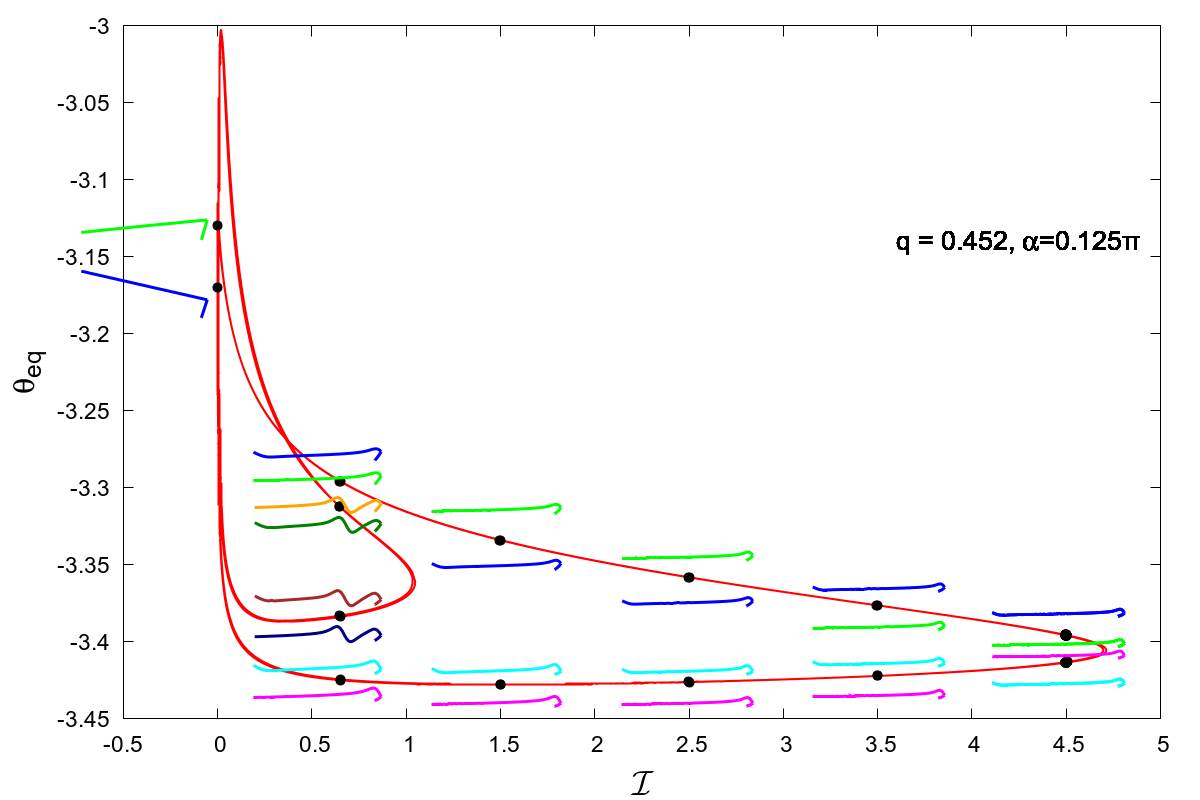
\includegraphics[width=0.9\textwidth]{plots/combine_elastic_beam_I_theta_q_0.452_alpha_0.125pi_initial_-4.80_0_step.png}
		\end{center}
		%	\setlength{\abovecaptionskip}{-0.5 cm}
	\end{figure}\vspace{-0.3cm}
	%\selectfont \fontsize{10}{15}\selectfont
	\bi
	\item 4 branches in the line.
	\item "Higher modes" appear in deformations.
	\ei
	\end{overlayarea}
\end{frame}

%%%%%%%%%%%%%%%%%%%%%%%%%%%%%%%%%%%%%%%%%%%%%%%%%%%%%%%%%%%%%%%%%%%%%%




\begin{frame}
	\frametitle{Results (larger $q$): it gets even messy.}
	\begin{overlayarea}{\textwidth}{\textheight}\vspace{-0.3cm}
		\begin{figure}[htb]
			\begin{center}
				% specify width as 80% of the width of the text on the page
				% we can also specify a width in centimetres, e.g. [width=8cm]
				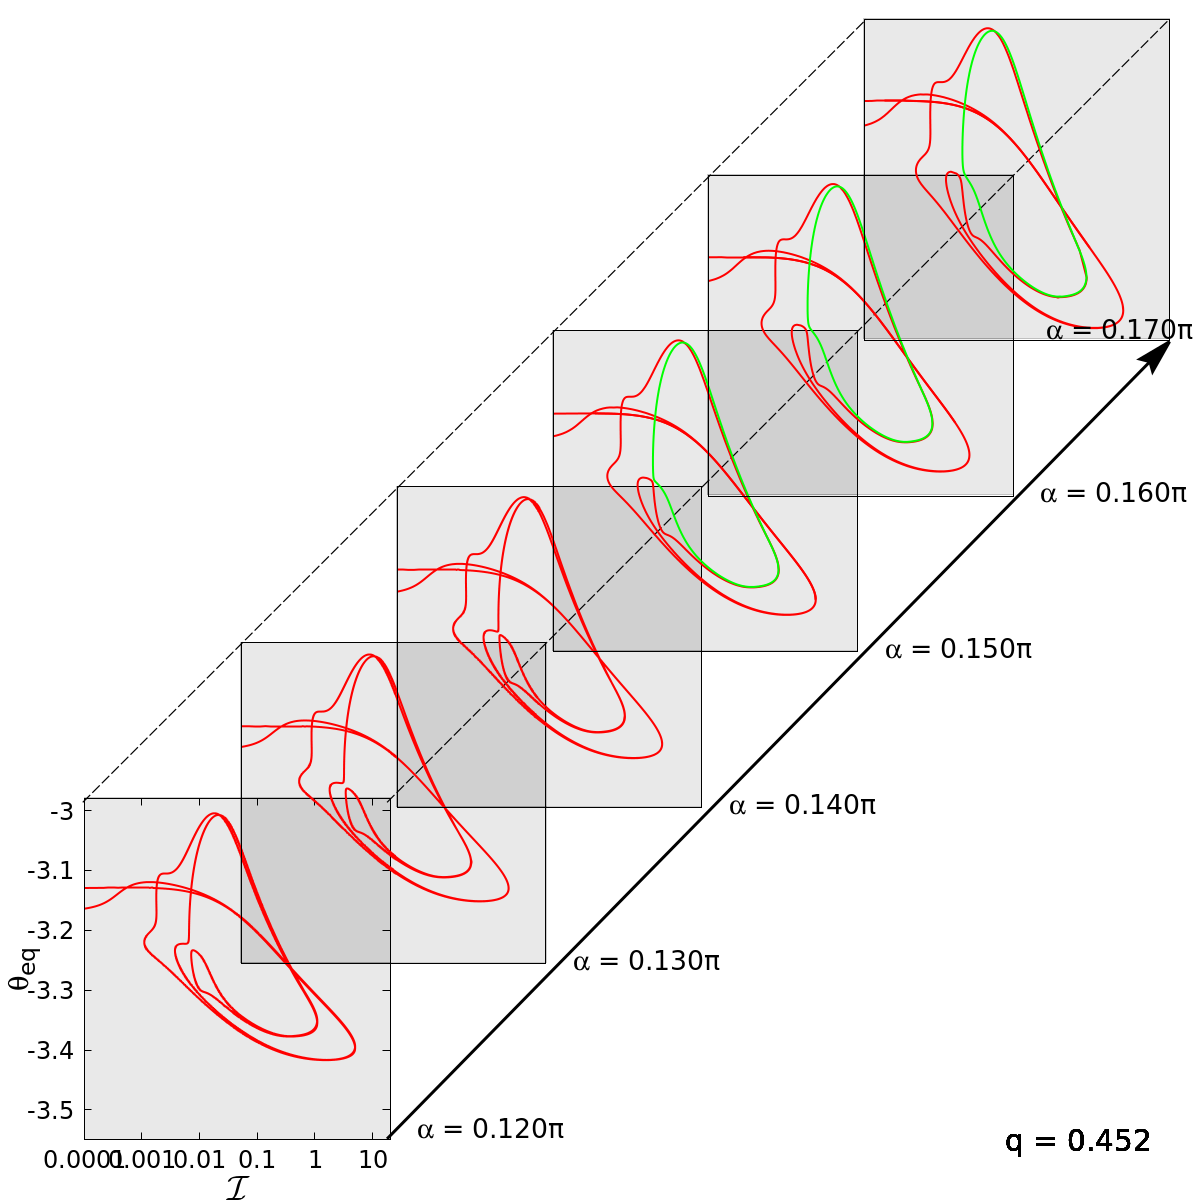
\includegraphics[width=0.65\textwidth]{plots/elastic_beam_I_theta_q_0.452_alpha_restart1.png}
			\end{center}
			%	\setlength{\abovecaptionskip}{-0.5 cm}
		\end{figure}\vspace{-0.3cm}
	\bi
	\item More disconnected loops.
	\ei 
		%\selectfont \fontsize{10}{15}\selectfont
	\end{overlayarea}
\end{frame}

%%%%%%%%%%%%%%%%%%%%%%%%%%%%%%%%%%%%%%%%%%%%%%%%%%%%%%%%%%%%%%%%%%%%%%


\begin{frame}
	\frametitle{Results (larger $q$): it gets even messy.}
	\begin{overlayarea}{\textwidth}{\textheight}\vspace{-0.3cm}
		\begin{figure}[htb]
			\begin{center}
				% specify width as 80% of the width of the text on the page
				% we can also specify a width in centimetres, e.g. [width=8cm]
				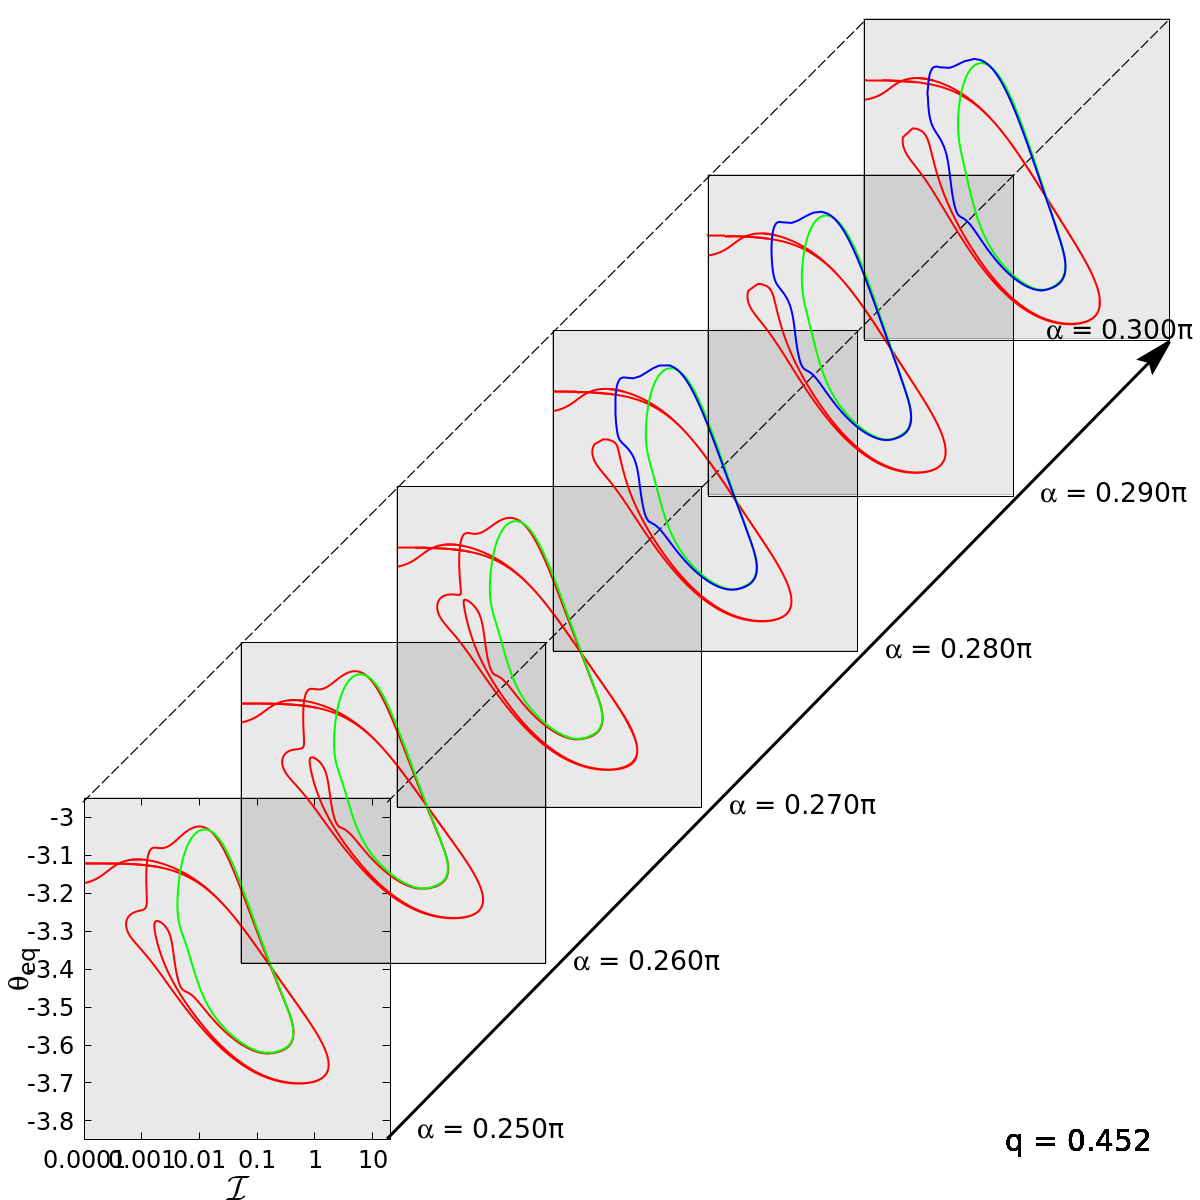
\includegraphics[width=0.65\textwidth]{plots/elastic_beam_I_theta_q_0.452_alpha_restart2.png}
			\end{center}
			%	\setlength{\abovecaptionskip}{-0.5 cm}
		\end{figure}\vspace{-0.3cm}
		\bi
		\item More disconnected loops.
		\ei 
		%\selectfont \fontsize{10}{15}\selectfont
	\end{overlayarea}
\end{frame}


%%%%%%%%%%%%%%%%%%%%%%%%%%%%%%%%%%%%%%%%%%%%%%%%%%%%%%%%%%%%%%%%%%%%%%


\begin{frame}
	\frametitle{Results (larger $q$): it gets even messy.}
	\begin{overlayarea}{\textwidth}{\textheight}\vspace{-0.3cm}
		\begin{figure}[htb]
			\begin{center}
				% specify width as 80% of the width of the text on the page
				% we can also specify a width in centimetres, e.g. [width=8cm]
				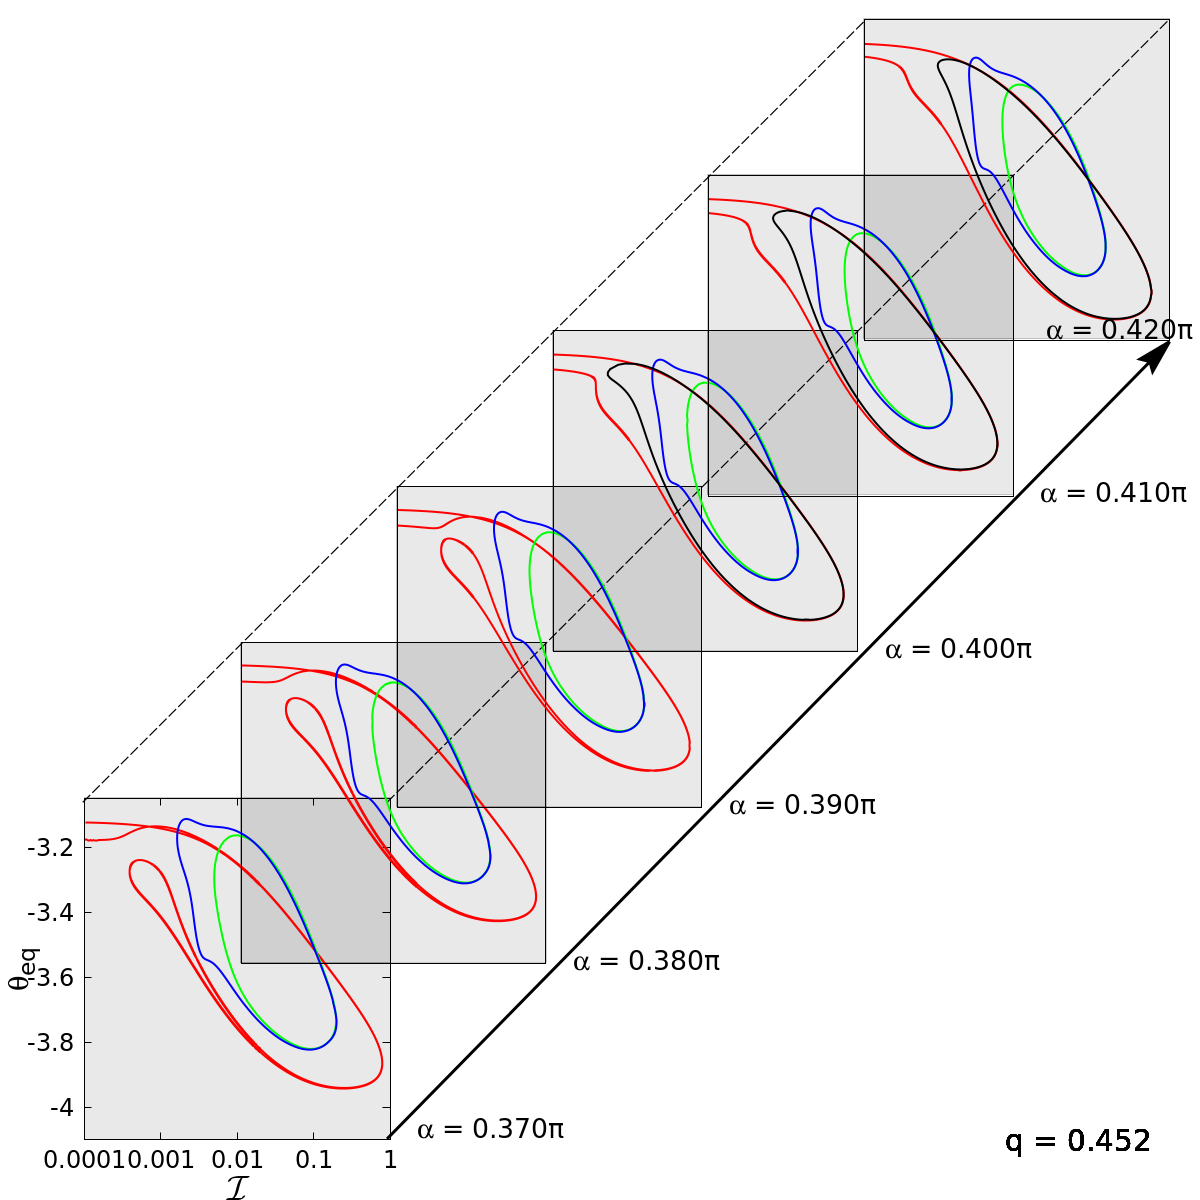
\includegraphics[width=0.65\textwidth]{plots/elastic_beam_I_theta_q_0.452_alpha_restart3.png}
			\end{center}
			%	\setlength{\abovecaptionskip}{-0.5 cm}
		\end{figure}\vspace{-0.3cm}
		\bi
		\item More disconnected loops.
		\ei 
		%\selectfont \fontsize{10}{15}\selectfont
	\end{overlayarea}
\end{frame}

%%%%%%%%%%%%%%%%%%%%%%%%%%%%%%%%%%%%%%%%%%%%%%%%%%%%%%%%%%%%%%%%%%%%%%

\begin{frame}
	\frametitle{Results: shapes}
	\begin{overlayarea}{\textwidth}{\textheight}
\begin{itemize}
	\item Classify four types of shapes: \vspace{-0.3cm}
	\begin{figure}[htb]
		\begin{center}
			% specify width as 80% of the width of the text on the page
			% we can also specify a width in centimetres, e.g. [width=8cm]
			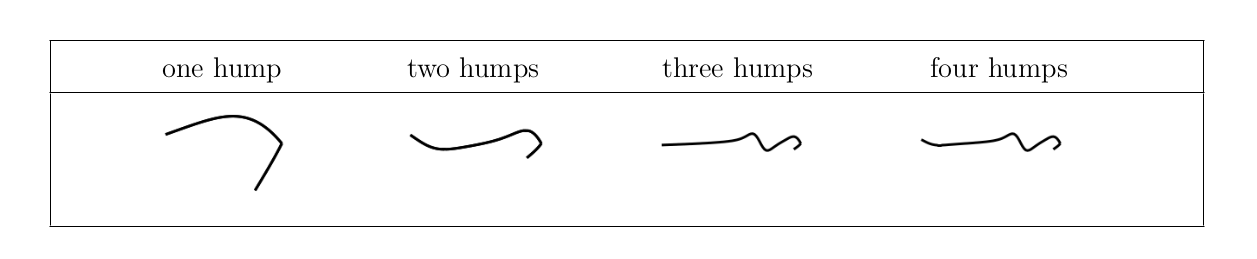
\includegraphics[width=1\textwidth]{plots/deformations.png}
		\end{center}
		%	\setlength{\abovecaptionskip}{-0.5 cm}
	\end{figure}
	%\selectfont \fontsize{10}{15}\selectfont
\end{itemize}
	\end{overlayarea}
\end{frame}



%%%%%%%%%%%%%%%%%%%%%%%%%%%%%%%%%%%%%%%%%%%%%%%%%%%%%%%%%%%%%%%%%%%%%%

%%%%%%%%%%%%%%%%%%%%%%%%%%%%%%%%%%%%%%%%%%%%%%%%%%%%%%%%%%%%%%%%%%%%%%


\begin{frame}
	\frametitle{Results: shapes}
	\begin{overlayarea}{\textwidth}{\textheight}
		\begin{itemize}
			\item Classify four types of shapes: \vspace{-0.3cm}
			\begin{figure}[htb]
				\begin{center}
					% specify width as 80% of the width of the text on the page
					% we can also specify a width in centimetres, e.g. [width=8cm]
					\includegraphics[width=1\textwidth]{plots/deformations.png}
				\end{center}
				%	\setlength{\abovecaptionskip}{-0.5 cm}
			\end{figure}
			\item Is this Euler buckling?
			\item Is the beam subject to compression?
			%\selectfont \fontsize{10}{15}\selectfont
		\end{itemize}
	\end{overlayarea}
\end{frame}



%%%%%%%%%%%%%%%%%%%%%%%%%%%%%%%%%%%%%%%%%%%%%%%%%%%%%%%%%%%%%%%%%%%%%%


\begin{frame}
	\frametitle{Results: analysis of tensile stress.}
	\begin{overlayarea}{\textwidth}{\textheight}
		\vspace{-0.3cm}
	\begin{itemize}
		\item \small Tensile stress in beam:
		\begin{equation*}
			\sigma(\xi)=\int_0^\xi (\mathbf{f}\cdot\mathbf{e}_t) \left |\frac{\partial \mathbf{R}}{\partial \xi}\right|\,d\xi,
		\end{equation*}
		where $\mathbf{e}_t$ is the unit tangent vector to the surface of the particle. 
	\item \small Therefore, we have 
	\begin{equation*}\small 
		\sigma(\xi)=\left\{
		\begin{aligned}
			\label{eq:4}
			&\int_0^\xi (\mathbf{f}\cdot\mathbf{e}_{t1}) \left |\frac{\partial \mathbf{R}}{\partial \xi}\right|\,d\xi,\quad \xi\in[0,0.5-q];\\
			&-\mathbf{F}_2\cdot\mathbf{e}_{t2}+\int_{0.5-q}^\xi (\mathbf{f}\cdot\mathbf{e}_{t2}) \left |\frac{\partial \mathbf{R}}{\partial \xi}\right|\,d\xi, \quad \xi\in[0.5-q,1].
		\end{aligned}\right.
	\end{equation*}
	\end{itemize}\vspace{-0.4cm}
	\begin{figure}[htb]
	\begin{center}
		% specify width as 80% of the width of the text on the page
		% we can also specify a width in centimetres, e.g. [width=8cm]
		\includegraphics[width=0.55\textwidth]{plots/tensile_boomerang.png}
	\end{center}
	%	\setlength{\abovecaptionskip}{-0.5 cm}
\end{figure}
	\end{overlayarea}
\end{frame}

%%%%%%%%%%%%%%%%%%%%%%%%%%%%%%%%%%%%%%%%%%%%%%%%%%%%%%%%%%%%%%%%%%%%%%

\begin{frame}
	\frametitle{Results: tensile stress.}
	\begin{overlayarea}{\textwidth}{\textheight}
Tensile stress for different shape parameters ($\mathcal{I}=0$).\vspace{-0.2cm}
\begin{figure}[!h]
	\centering
	\subfigure[\tiny $q=0.35,\alpha=0.125\pi$]{
		\begin{minipage}[b]{0.25\textwidth}
			\includegraphics[width=1\textwidth]{plots/sigma_q_0.35_alpha_0.125pi.png} 
		\end{minipage}
		\label{fig:10.a}
	}
	\subfigure[\tiny $q=0.40,\alpha=0.125\pi$]{
		\begin{minipage}[b]{0.25\textwidth}
			\includegraphics[width=1\textwidth]{plots/sigma_q_0.40_alpha_0.125pi.png}
		\end{minipage}
		\label{fig:10.b}
	}
	\subfigure[\tiny $q=0.45,\alpha=0.125\pi$]{
		\begin{minipage}[b]{0.25\textwidth}
			\includegraphics[width=1\textwidth]{plots/sigma_q_0.45_alpha_0.125pi.png}
		\end{minipage}
		\label{fig:10.c}
	}
	\\ 
	\subfigure[\tiny $q=0.35,\alpha=0.25\pi$]{
		\begin{minipage}[b]{0.25\textwidth}
			\includegraphics[width=1\textwidth]{plots/sigma_q_0.35_alpha_0.250pi.png} 
		\end{minipage}
		\label{fig:10.d}
	}
	\subfigure[\tiny $q=0.40,\alpha=0.25\pi$]{
		\begin{minipage}[b]{0.25\textwidth}
			\includegraphics[width=1\textwidth]{plots/sigma_q_0.40_alpha_0.250pi.png}
		\end{minipage}
		\label{fig:10.e}
	}
	\subfigure[\tiny $q=0.45,\alpha=0.25\pi$]{
		\begin{minipage}[b]{0.25\textwidth}
			\includegraphics[width=1\textwidth]{plots/sigma_q_0.45_alpha_0.250pi.png}
		\end{minipage}
		\label{fig:10.f}
	}
\end{figure}
	\end{overlayarea}
\end{frame}

%%%%%%%%%%%%%%%%%%%%%%%%%%%%%%%%%%%%%%%%%%%%%%%%%%%%%%%%%%%%%%%%%%%%%%


\begin{frame}
	\frametitle{Summary}
	\begin{overlayarea}{\textwidth}{\textheight}
	\bi
	\item Consider the case of a single elastic particle in shear flow, as its motion is primarily governed by the background flow, not by interactions with other particles.
	\item Two of the four fixed orientations differ by an angle of $\pi$, but share the same shape.
	\item Initial configuration ($q,\alpha$) plays an important role in deformations.
	\item Four types of deformations observed.
	\item If the short arm is relative small, varying $\alpha$ may cause a bifurcation, creating a new closed loop in the steady orientation vs. FSI coefficient plot.
	\item No matter how complex the curve becomes, it always starts and ends at $\mathcal{I}=0$.
	\ei
	\end{overlayarea}
\end{frame}

%%%%%%%%%%%%%%%%%%%%%%%%%%%%%%%%%%%%%%%%%%%%%%%%%%%%%%%%%%%%%%%%%%%%%%
\begin{frame}
\begin{overlayarea}{\textwidth}{\textheight}
	\frametitle{Bibliography}
	\small
\bibliography{references}
\end{overlayarea}
\end{frame}
%%%%%%%%%%%%%%%%%%%%%%%%%%%%%%%%%%%%%%%%%%%%%%%%%%%%%%%%%%%%%%%%%%%%%%

\begin{frame}
	\frametitle{Brief introduction of finite element method}
	\begin{overlayarea}{\textwidth}{\textheight}
		%\vspace{-0.8cm}
		%	\begin{columns}
			%	\column{.5\textwidth}
			Let us consider a 1D problem: $\mathcal{R}(x;u(x))=0$, for $ x\in [0,1]$ subject to $u(x=0)=g_0, u(x=1)=g_1$.
			\small\bi
			\item Split the solution into two parts (Galerkin method): \vspace{-0.2cm}$$u(x)=u_p(x)+u_h(x)=u_p(x)+\sum^{N-1}_{j=2}U_j\psi_j(x).$$
			($u_p(x=0)=g_0,u_p(x=1)=g_1$; $u_h(x=0)=u_h(x=1)=0$.)
			\item Weak formulation (weak solution satisfies equation almost everywhere of domain): $$r_k(U_2,U_3,...,U_{N-1})=\int^1_0\mathcal{R}\Bigg(u_p(x)+\sum^{N-1}_{j=2}U_j\psi_j(x)\Bigg)\,\psi_k(x)\,dx.$$
			\item Note that $\{U_2,U_3,...U_{N-1}\}$ are the unknowns. 
			\ei
			
			
			%\column{.5\textwidth}
			
			%\end{columns}
		\end{overlayarea}
	\end{frame}
	
	%%%%%%%%%%%%%%%%%%%%%%%%%%%%%%%%%%%%%%%%%%%%%%%%%%%%%%%%%%%%%%%%%%%%%%
	
	
	
	\begin{frame}
		\frametitle{Brief introduction of finite element method}
		\begin{overlayarea}{\textwidth}{\textheight}
			\vspace{-0.2cm}\small	Shape functions: "hat functions".
			$$\psi_j(x)=
			\begin{cases}
				0 & \text{for}\quad x<X_{j-1} \\
				\frac{x-X_{j-1}}{X_{j}-X_{j-1}} & \text{for}\quad X_{j-1}<x<X_{j}\\
				\frac{X_{j+1}-x}{X_{j+1}-X_{j}} & \text{for}\quad X_{j}<x<X_{j+1} \\
				0 & \text{for}\quad x>X_{j+1}
			\end{cases}$$\vspace{-0.6cm}
			\begin{figure}[htb]
				\begin{minipage}[t]{0.49\linewidth}
					\centering
					\includegraphics[scale=0.22]{plots/finite1.png}
				\end{minipage}
				\begin{minipage}[t]{0.49\linewidth}
					\centering
					\includegraphics[scale=0.22]{plots/finite2.png}
				\end{minipage}
			\end{figure}\vspace{-0.2cm}
			\bi
			\item Shape functions satisfy $\psi_j(X_i)=
			\begin{cases}
				1 & \text{if}\quad i=j \\
				0 & \text{for}\quad i\neq j
			\end{cases}.$
			\item Piecewise linear interpolation $v(x)=\sum^N_{j=1} V_j \psi_j(x)$.
			\ei
		\end{overlayarea}
	\end{frame}
	
	%%%%%%%%%%%%%%%%%%%%%%%%%%%%%%%%%%%%%%%%%%%%%%%%%%%%%%%%%%%%%%%%%%%%%%
	
	
	
	\begin{frame}
		\frametitle{Newton method}
		\begin{overlayarea}{\textwidth}{\textheight}
			\vspace{-0.5cm}\small	
			\bi
			\item Set $u_p=g_0\psi_1(x)+g_1\psi_N(x)$ and $\sum^{N-1}_{j=2}U_j\psi_j(x)$.
			\item Provide an initial guess for the unknowns $\{U_2,U_3,...U_{N-1}\}$, denoted as $U_i^{(0)}, i=2,...,N-1.$
			\item Determine the residuals $$r_k^{(0)}=\int^1_0\mathcal{R}\Bigg(u_p(x)+\sum^{N-1}_{j=2}U_j\psi_j(x)\Bigg)\,\psi_k(x)\,dx,\, k=2,...,N-1.$$
			and the entries in the Jacobian matrix $J_{kj}=\frac{\partial r_k}{\partial U_j},\, k,j=2,...,N-1.$
			\item Solve the linear system $\sum^{N-1}_{j=2}J_{kj}\,\delta U_j=-r_k^{(0)},\,k=2,...,N-1.$
			\item Correct the initial guess via $U_j=U_j^{(0)}+\delta U_j,\, j=2,...,N-1.$ 
			\item The finite-element solution is\vspace{-0.2cm} $$u^{(FE)}(x)=g_0\psi_1(x)+g_1\psi_N(x)+\sum^{N-1}_{j=2}U_j\psi_j(x).$$
			\ei
		\end{overlayarea}
	\end{frame}
	
	%%%%%%%%%%%%%%%%%%%%%%%%%%%%%%%%%%%%%%%%%%%%%%%%%%%%%%%%%%%%%%%%%%%%%%

\end{document}


